%% bare_jrnl_compsoc.tex
%% V1.4b
%% 2015/08/26
%% by Michael Shell
%% See:
%% http://www.michaelshell.org/
%% for current contact information.
%%
%% This is a skeleton file demonstrating the use of IEEEtran.cls
%% (requires IEEEtran.cls version 1.8b or later) with an IEEE
%% Computer Society journal paper.
%%
%% Support sites:
%% http://www.michaelshell.org/tex/ieeetran/
%% http://www.ctan.org/pkg/ieeetran
%% and
%% http://www.ieee.org/

%%*************************************************************************
%% Legal Notice:
%% This code is offered as-is without any warranty either expressed or
%% implied; without even the implied warranty of MERCHANTABILITY or
%% FITNESS FOR A PARTICULAR PURPOSE! 
%% User assumes all risk.
%% In no event shall the IEEE or any contributor to this code be liable for
%% any damages or losses, including, but not limited to, incidental,
%% consequential, or any other damages, resulting from the use or misuse
%% of any information contained here.
%%
%% All comments are the opinions of their respective authors and are not
%% necessarily endorsed by the IEEE.
%%
%% This work is distributed under the LaTeX Project Public License (LPPL)
%% ( http://www.latex-project.org/ ) version 1.3, and may be freely used,
%% distributed and modified. A copy of the LPPL, version 1.3, is included
%% in the base LaTeX documentation of all distributions of LaTeX released
%% 2003/12/01 or later.
%% Retain all contribution notices and credits.
%% ** Modified files should be clearly indicated as such, including  **
%% ** renaming them and changing author support contact information. **
%%*************************************************************************


% *** Authors should verify (and, if needed, correct) their LaTeX system  ***
% *** with the testflow diagnostic prior to trusting their LaTeX platform ***
% *** with production work. The IEEE's font choices and paper sizes can   ***
% *** trigger bugs that do not appear when using other class files.       ***                          ***
% The testflow support page is at:
% http://www.michaelshell.org/tex/testflow/


\documentclass[10pt,journal,compsoc]{IEEEtran}
%
% If IEEEtran.cls has not been installed into the LaTeX system files,
% manually specify the path to it like:
% \documentclass[10pt,journal,compsoc]{../sty/IEEEtran}





% Some very useful LaTeX packages include:
% (uncomment the ones you want to load)


% *** MISC UTILITY PACKAGES ***
%
%\usepackage{ifpdf}
% Heiko Oberdiek's ifpdf.sty is very useful if you need conditional
% compilation based on whether the output is pdf or dvi.
% usage:
% \ifpdf
%   % pdf code
% \else
%   % dvi code
% \fi
% The latest version of ifpdf.sty can be obtained from:
% http://www.ctan.org/pkg/ifpdf
% Also, note that IEEEtran.cls V1.7 and later provides a builtin
% \ifCLASSINFOpdf conditional that works the same way.
% When switching from latex to pdflatex and vice-versa, the compiler may
% have to be run twice to clear warning/error messages.






% *** CITATION PACKAGES ***
%
\ifCLASSOPTIONcompsoc
  % IEEE Computer Society needs nocompress option
  % requires cite.sty v4.0 or later (November 2003)
  \usepackage[nocompress]{cite}
\else
  % normal IEEE
  \usepackage{cite}
\fi
% cite.sty was written by Donald Arseneau
% V1.6 and later of IEEEtran pre-defines the format of the cite.sty package
% \cite{} output to follow that of the IEEE. Loading the cite package will
% result in citation numbers being automatically sorted and properly
% "compressed/ranged". e.g., [1], [9], [2], [7], [5], [6] without using
% cite.sty will become [1], [2], [5]--[7], [9] using cite.sty. cite.sty's
% \cite will automatically add leading space, if needed. Use cite.sty's
% noadjust option (cite.sty V3.8 and later) if you want to turn this off
% such as if a citation ever needs to be enclosed in parenthesis.
% cite.sty is already installed on most LaTeX systems. Be sure and use
% version 5.0 (2009-03-20) and later if using hyperref.sty.
% The latest version can be obtained at:
% http://www.ctan.org/pkg/cite
% The documentation is contained in the cite.sty file itself.
%
% Note that some packages require special options to format as the Computer
% Society requires. In particular, Computer Society  papers do not use
% compressed citation ranges as is done in typical IEEE papers
% (e.g., [1]-[4]). Instead, they list every citation separately in order
% (e.g., [1], [2], [3], [4]). To get the latter we need to load the cite
% package with the nocompress option which is supported by cite.sty v4.0
% and later. Note also the use of a CLASSOPTION conditional provided by
% IEEEtran.cls V1.7 and later.





% *** GRAPHICS RELATED PACKAGES ***
%
\ifCLASSINFOpdf
  \usepackage[pdftex]{graphicx}
  % declare the path(s) where your graphic files are
  \graphicspath{{figs/}}
  % and their extensions so you won't have to specify these with
  % every instance of \includegraphics
  \DeclareGraphicsExtensions{.pdf,.jpeg,.png,.jpg}
\else
  % or other class option (dvipsone, dvipdf, if not using dvips). graphicx
  % will default to the driver specified in the system graphics.cfg if no
  % driver is specified.
  % \usepackage[dvips]{graphicx}
  % declare the path(s) where your graphic files are
  % \graphicspath{{../figs/}}
  % and their extensions so you won't have to specify these with
  % every instance of \includegraphics
  % \DeclareGraphicsExtensions{.eps}
\fi
% graphicx was written by David Carlisle and Sebastian Rahtz. It is
% required if you want graphics, photos, etc. graphicx.sty is already
% installed on most LaTeX systems. The latest version and documentation
% can be obtained at: 
% http://www.ctan.org/pkg/graphicx
% Another good source of documentation is "Using Imported Graphics in
% LaTeX2e" by Keith Reckdahl which can be found at:
% http://www.ctan.org/pkg/epslatex
%
% latex, and pdflatex in dvi mode, support graphics in encapsulated
% postscript (.eps) format. pdflatex in pdf mode supports graphics
% in .pdf, .jpeg, .png and .mps (metapost) formats. Users should ensure
% that all non-photo figures use a vector format (.eps, .pdf, .mps) and
% not a bitmapped formats (.jpeg, .png). The IEEE frowns on bitmapped formats
% which can result in "jaggedy"/blurry rendering of lines and letters as
% well as large increases in file sizes.
%
% You can find documentation about the pdfTeX application at:
% http://www.tug.org/applications/pdftex






% *** MATH PACKAGES ***
%
%\usepackage{amsmath}
% A popular package from the American Mathematical Society that provides
% many useful and powerful commands for dealing with mathematics.
%
% Note that the amsmath package sets \interdisplaylinepenalty to 10000
% thus preventing page breaks from occurring within multiline equations. Use:
%\interdisplaylinepenalty=2500
% after loading amsmath to restore such page breaks as IEEEtran.cls normally
% does. amsmath.sty is already installed on most LaTeX systems. The latest
% version and documentation can be obtained at:
% http://www.ctan.org/pkg/amsmath





% *** SPECIALIZED LIST PACKAGES ***
%
%\usepackage{algorithmic}
% algorithmic.sty was written by Peter Williams and Rogerio Brito.
% This package provides an algorithmic environment fo describing algorithms.
% You can use the algorithmic environment in-text or within a figure
% environment to provide for a floating algorithm. Do NOT use the algorithm
% floating environment provided by algorithm.sty (by the same authors) or
% algorithm2e.sty (by Christophe Fiorio) as the IEEE does not use dedicated
% algorithm float types and packages that provide these will not provide
% correct IEEE style captions. The latest version and documentation of
% algorithmic.sty can be obtained at:
% http://www.ctan.org/pkg/algorithms
% Also of interest may be the (relatively newer and more customizable)
% algorithmicx.sty package by Szasz Janos:
% http://www.ctan.org/pkg/algorithmicx




% *** ALIGNMENT PACKAGES ***
%
\usepackage{array}
% Frank Mittelbach's and David Carlisle's array.sty patches and improves
% the standard LaTeX2e array and tabular environments to provide better
% appearance and additional user controls. As the default LaTeX2e table
% generation code is lacking to the point of almost being broken with
% respect to the quality of the end results, all users are strongly
% advised to use an enhanced (at the very least that provided by array.sty)
% set of table tools. array.sty is already installed on most systems. The
% latest version and documentation can be obtained at:
% http://www.ctan.org/pkg/array


% IEEEtran contains the IEEEeqnarray family of commands that can be used to
% generate multiline equations as well as matrices, tables, etc., of high
% quality.




% *** SUBFIGURE PACKAGES ***
%\ifCLASSOPTIONcompsoc
%  \usepackage[caption=false,font=footnotesize,labelfont=sf,textfont=sf]{subfig}
%\else
%  \usepackage[caption=false,font=footnotesize]{subfig}
%\fi
% subfig.sty, written by Steven Douglas Cochran, is the modern replacement
% for subfigure.sty, the latter of which is no longer maintained and is
% incompatible with some LaTeX packages including fixltx2e. However,
% subfig.sty requires and automatically loads Axel Sommerfeldt's caption.sty
% which will override IEEEtran.cls' handling of captions and this will result
% in non-IEEE style figure/table captions. To prevent this problem, be sure
% and invoke subfig.sty's "caption=false" package option (available since
% subfig.sty version 1.3, 2005/06/28) as this is will preserve IEEEtran.cls
% handling of captions.
% Note that the Computer Society format requires a sans serif font rather
% than the serif font used in traditional IEEE formatting and thus the need
% to invoke different subfig.sty package options depending on whether
% compsoc mode has been enabled.
%
% The latest version and documentation of subfig.sty can be obtained at:
% http://www.ctan.org/pkg/subfig




% *** FLOAT PACKAGES ***
%
%\usepackage{fixltx2e}
% fixltx2e, the successor to the earlier fix2col.sty, was written by
% Frank Mittelbach and David Carlisle. This package corrects a few problems
% in the LaTeX2e kernel, the most notable of which is that in current
% LaTeX2e releases, the ordering of single and double column floats is not
% guaranteed to be preserved. Thus, an unpatched LaTeX2e can allow a
% single column figure to be placed prior to an earlier double column
% figure.
% Be aware that LaTeX2e kernels dated 2015 and later have fixltx2e.sty's
% corrections already built into the system in which case a warning will
% be issued if an attempt is made to load fixltx2e.sty as it is no longer
% needed.
% The latest version and documentation can be found at:
% http://www.ctan.org/pkg/fixltx2e


%\usepackage{stfloats}
% stfloats.sty was written by Sigitas Tolusis. This package gives LaTeX2e
% the ability to do double column floats at the bottom of the page as well
% as the top. (e.g., "\begin{figure*}[!b]" is not normally possible in
% LaTeX2e). It also provides a command:
%\fnbelowfloat
% to enable the placement of footnotes below bottom floats (the standard
% LaTeX2e kernel puts them above bottom floats). This is an invasive package
% which rewrites many portions of the LaTeX2e float routines. It may not work
% with other packages that modify the LaTeX2e float routines. The latest
% version and documentation can be obtained at:
% http://www.ctan.org/pkg/stfloats
% Do not use the stfloats baselinefloat ability as the IEEE does not allow
% \baselineskip to stretch. Authors submitting work to the IEEE should note
% that the IEEE rarely uses double column equations and that authors should try
% to avoid such use. Do not be tempted to use the cuted.sty or midfloat.sty
% packages (also by Sigitas Tolusis) as the IEEE does not format its papers in
% such ways.
% Do not attempt to use stfloats with fixltx2e as they are incompatible.
% Instead, use Morten Hogholm'a dblfloatfix which combines the features
% of both fixltx2e and stfloats:
%
% \usepackage{dblfloatfix}
% The latest version can be found at:
% http://www.ctan.org/pkg/dblfloatfix




%\ifCLASSOPTIONcaptionsoff
%  \usepackage[nomarkers]{endfloat}
% \let\MYoriglatexcaption\caption
% \renewcommand{\caption}[2][\relax]{\MYoriglatexcaption[#2]{#2}}
%\fi
% endfloat.sty was written by James Darrell McCauley, Jeff Goldberg and 
% Axel Sommerfeldt. This package may be useful when used in conjunction with 
% IEEEtran.cls'  captionsoff option. Some IEEE journals/societies require that
% submissions have lists of figures/tables at the end of the paper and that
% figures/tables without any captions are placed on a page by themselves at
% the end of the document. If needed, the draftcls IEEEtran class option or
% \CLASSINPUTbaselinestretch interface can be used to increase the line
% spacing as well. Be sure and use the nomarkers option of endfloat to
% prevent endfloat from "marking" where the figures would have been placed
% in the text. The two hack lines of code above are a slight modification of
% that suggested by in the endfloat docs (section 8.4.1) to ensure that
% the full captions always appear in the list of figures/tables - even if
% the user used the short optional argument of \caption[]{}.
% IEEE papers do not typically make use of \caption[]'s optional argument,
% so this should not be an issue. A similar trick can be used to disable
% captions of packages such as subfig.sty that lack options to turn off
% the subcaptions:
% For subfig.sty:
% \let\MYorigsubfloat\subfloat
% \renewcommand{\subfloat}[2][\relax]{\MYorigsubfloat[]{#2}}
% However, the above trick will not work if both optional arguments of
% the \subfloat command are used. Furthermore, there needs to be a
% description of each subfigure *somewhere* and endfloat does not add
% subfigure captions to its list of figures. Thus, the best approach is to
% avoid the use of subfigure captions (many IEEE journals avoid them anyway)
% and instead reference/explain all the subfigures within the main caption.
% The latest version of endfloat.sty and its documentation can obtained at:
% http://www.ctan.org/pkg/endfloat
%
% The IEEEtran \ifCLASSOPTIONcaptionsoff conditional can also be used
% later in the document, say, to conditionally put the References on a 
% page by themselves.




% *** PDF, URL AND HYPERLINK PACKAGES ***
%
%\usepackage{url}
% url.sty was written by Donald Arseneau. It provides better support for
% handling and breaking URLs. url.sty is already installed on most LaTeX
% systems. The latest version and documentation can be obtained at:
% http://www.ctan.org/pkg/url
% Basically, \url{my_url_here}.





% *** Do not adjust lengths that control margins, column widths, etc. ***
% *** Do not use packages that alter fonts (such as pslatex).         ***
% There should be no need to do such things with IEEEtran.cls V1.6 and later.
% (Unless specifically asked to do so by the journal or conference you plan
% to submit to, of course. )

\usepackage{xcolor}

% correct bad hyphenation here
\hyphenation{op-tical net-works semi-conduc-tor}


\begin{document}
%
% paper title
% Titles are generally capitalized except for words such as a, an, and, as,
% at, but, by, for, in, nor, of, on, or, the, to and up, which are usually
% not capitalized unless they are the first or last word of the title.
% Linebreaks \\ can be used within to get better formatting as desired.
% Do not put math or special symbols in the title.
\title{CyberHaptics--\\
 Magnetic Implants as Haptic Devices}
%
%
% author names and IEEE memberships
% note positions of commas and nonbreaking spaces ( ~ ) LaTeX will not break
% a structure at a ~ so this keeps an author's name from being broken across
% two lines.
% use \thanks{} to gain access to the first footnote area
% a separate \thanks must be used for each paragraph as LaTeX2e's \thanks
% was not built to handle multiple paragraphs
%
%
%\IEEEcompsocitemizethanks is a special \thanks that produces the bulleted
% lists the Computer Society journals use for "first footnote" author
% affiliations. Use \IEEEcompsocthanksitem which works much like \item
% for each affiliation group. When not in compsoc mode,
% \IEEEcompsocitemizethanks becomes like \thanks and
% \IEEEcompsocthanksitem becomes a line break with idention. This
% facilitates dual compilation, although admittedly the differences in the
% desired content of \author between the different types of papers makes a
% one-size-fits-all approach a daunting prospect. For instance, compsoc 
% journal papers have the author affiliations above the "Manuscript
% received ..."  text while in non-compsoc journals this is reversed. Sigh.

\author{Axel Fougues and Abderrahmane Kheddar,~\IEEEmembership{Senior~Member,~IEEE}% <-this % stops a space
\IEEEcompsocitemizethanks{\IEEEcompsocthanksitem A. Fougues and A. Kheddar are with the CNRS-University of Montpellier, LIRMM, Montpellier, France.\protect\\
% note need leading \protect in front of \\ to get a newline within \thanks as
% \\ is fragile and will error, could use \hfil\break instead.
E-mail: see http://www.michaelshell.org/contact.html
\IEEEcompsocthanksitem A. Kheddar is also with the CNRS-AIST Joint Robotics Laboratory, Tsukuba, Japan.}% <-this % stops an unwanted space
\thanks{Manuscript received July X, 2021; revised Y 00, 202X.}}

% note the % following the last \IEEEmembership and also \thanks - 
% these prevent an unwanted space from occurring between the last author name
% and the end of the author line. i.e., if you had this:
% 
% \author{....lastname \thanks{...} \thanks{...} }
%                     ^------------^------------^----Do not want these spaces!
%
% a space would be appended to the last name and could cause every name on that
% line to be shifted left slightly. This is one of those "LaTeX things". For
% instance, "\textbf{A} \textbf{B}" will typeset as "A B" not "AB". To get
% "AB" then you have to do: "\textbf{A}\textbf{B}"
% \thanks is no different in this regard, so shield the last } of each \thanks
% that ends a line with a % and do not let a space in before the next \thanks.
% Spaces after \IEEEmembership other than the last one are OK (and needed) as
% you are supposed to have spaces between the names. For what it is worth,
% this is a minor point as most people would not even notice if the said evil
% space somehow managed to creep in.



% The paper headers
\markboth{IEEE Transactions on Haptics,~Vol.~X, No.~X, Xxxxxx~202X}%
{Fougues and Kheddar: Implants for Haptic}
% The only time the second header will appear is for the odd numbered pages
% after the title page when using the twoside option.
% 
% *** Note that you probably will NOT want to include the author's ***
% *** name in the headers of peer review papers.                   ***
% You can use \ifCLASSOPTIONpeerreview for conditional compilation here if
% you desire.



% The publisher's ID mark at the bottom of the page is less important with
% Computer Society journal papers as those publications place the marks
% outside of the main text columns and, therefore, unlike regular IEEE
% journals, the available text space is not reduced by their presence.
% If you want to put a publisher's ID mark on the page you can do it like
% this:
%\IEEEpubid{0000--0000/00\$00.00~\copyright~2015 IEEE}
% or like this to get the Computer Society new two part style.
%\IEEEpubid{\makebox[\columnwidth]{\hfill 0000--0000/00/\$00.00~\copyright~2015 IEEE}%
%\hspace{\columnsep}\makebox[\columnwidth]{Published by the IEEE Computer Society\hfill}}
% Remember, if you use this you must call \IEEEpubidadjcol in the second
% column for its text to clear the IEEEpubid mark (Computer Society jorunal
% papers don't need this extra clearance.)



% use for special paper notices
%\IEEEspecialpapernotice{(Invited Paper)}



% for Computer Society papers, we must declare the abstract and index terms
% PRIOR to the title within the \IEEEtitleabstractindextext IEEEtran
% command as these need to go into the title area created by \maketitle.
% As a general rule, do not put math, special symbols or citations
% in the abstract or keywords.
\IEEEtitleabstractindextext{%
\begin{abstract}
Haptic displays are multiple and diverse in technology. They can be found in the form of fixed, movable, portable, wearable, encounter-type and can display a subset of known haptic modalities. In this paper, we introduce a new category: human implant haptics. Implantable haptics conceptualizes the idea that haptic display systems can also be considered as permanent biocompatible implants in living organisms having touch sensing capabilities. They can be used to display haptic data or enhance perceptual modalities using surrounding nerf-endings. We specifically exemplify and investigate thus new concept, we termed cyberhaptics, with subcutaneous magnetic vibrator implants, and show how they can be used to convey haptic data or substituting non-haptic data into haptics.  
\end{abstract}

% Note that keywords are not normally used for peerreview papers.
\begin{IEEEkeywords}
Cyborg haptics, subcutaneous magnets, implant haptic displays.
\end{IEEEkeywords}}


% make the title area
\maketitle


% To allow for easy dual compilation without having to reenter the
% abstract/keywords data, the \IEEEtitleabstractindextext text will
% not be used in maketitle, but will appear (i.e., to be "transported")
% here as \IEEEdisplaynontitleabstractindextext when the compsoc 
% or transmag modes are not selected <OR> if conference mode is selected 
% - because all conference papers position the abstract like regular
% papers do.
\IEEEdisplaynontitleabstractindextext
% \IEEEdisplaynontitleabstractindextext has no effect when using
% compsoc or transmag under a non-conference mode.



% For peer review papers, you can put extra information on the cover
% page as needed:
% \ifCLASSOPTIONpeerreview
% \begin{center} \bfseries EDICS Category: 3-BBND \end{center}
% \fi
%
% For peerreview papers, this IEEEtran command inserts a page break and
% creates the second title. It will be ignored for other modes.
\IEEEpeerreviewmaketitle



\IEEEraisesectionheading{\section{Introduction}\label{sec:introduction}}
% Computer Society journal (but not conference!) papers do something unusual
% with the very first section heading (almost always called "Introduction").
% They place it ABOVE the main text! IEEEtran.cls does not automatically do
% this for you, but you can achieve this effect with the provided
% \IEEEraisesectionheading{} command. Note the need to keep any \label that
% is to refer to the section immediately after \section in the above as
% \IEEEraisesectionheading puts \section within a raised box.




% The very first letter is a 2 line initial drop letter followed
% by the rest of the first word in caps (small caps for compsoc).
% 
% form to use if the first word consists of a single letter:
% \IEEEPARstart{A}{demo} file is ....
% 
% form to use if you need the single drop letter followed by
% normal text (unknown if ever used by the IEEE):
% \IEEEPARstart{A}{}demo file is ....
% 
% Some journals put the first two words in caps:
% \IEEEPARstart{T}{his demo} file is ....
% 
% Here we have the typical use of a "T" for an initial drop letter
% and "HIS" in caps to complete the first word.
\IEEEPARstart{C}{yberhaptics}, a name composed from cybernetic or cyborg and haptics, designates any technology that enables providing or enhancing human haptics by implanting an artificial component of technology in a living organism. This type of haptic technology is not researched despite potential needs in terms of restoring human haptic sensations for amputees, and the new trend in human augmentation through various technologies (e.g. Google glass, mobile phones, etc.). Almost all existing haptic technologies are external devices that convey haptic data through direct contact on organism's skins. They can be found in the form of fixed or portable, graspable, wearable, touchable (encounter-type), pseudo-type and can display a subset of known haptic modalities, see recent reviews in~\cite{culbertson2018arcras}.  

It is however possible to envision haptic devices as bio-compatible fully or partially implantable devices that are permanently part of the human body. This novel research in cyborg haptics, that we named \emph{cyberhaptic technology} might offer tremendous perspectives and challenging investigations for new knowledge and applications. We are all cyborgs already as we relay and depends on several devices that enhance our perceptual, cognitive and strength capabilities. For being active by essence, haptic devices cannot be fully implantable as they still depend on an external source of information to be displayed. However, the mechanical transducer can be fully integrated and in various ways. In the future, we may expect advances in technology such that more sophisticated implants at different subcutaneous levels can serve the purpose of haptic displays to relay stealthily information. 

In this paper, we investigate the use of sub-dermal magnetic implants or SMIs(see Section~\ref{sec:background}). Magnetic implants appeared in the early 2010's among the biohacking community and have since vastly evolved both in design and uses. They consist of a strong magnet encapsulated in a biocompatible material and are usually implanted right beneath the skin in the hypo-dermis. These have found many uses over the years as practical tools, entertainment or wireless earphones. The ones we will be focusing on are particularly small and placed in the fingertips to give the user a sense of magnetic fields: when the implant interacts with an external field, it moves or vibrates among the user's nerve endings. This simple system provides the ability to detect, touch and identify fields with surprising precision as studied in depth by I. Harrison \cite{harrison2018tf}.

What we aim to prove is the feasibility of using implantable magnets as haptic rendering device in concrete use cases, like feedback for virtual and augmented reality. Assuming this is the case, magnetic implants would provide a mechanically simpler and potentially scale-able approach to haptic rendering. Most importantly they introduce the possibility of haptics through sub-dermal, permanent technologies.



\section{Background}
\label{sec:background}
\subsection{Sub-dermal implants and cutaneous mechanoreceptors}
Among the skin's mechanoreceptors, the nerve endings dedicated to tactile stimuli, it is the quickly adapting (QA) that are mostly involved in the perception of the implant (J. Hameed \cite{hameed2010ieee}). They are composed of Pacinian and Meissner corpuscles that are receptively sensitive to ranges of 200-300Hz and around 50Hz which loosely corresponds to the detectable frequency range of the implants \cite{hameed2010ieee}.

Since they interact with the mechanoreceptors directly or within internal soft tissue rather than through the epidermis, it is fair to expect a different response to a identical stimuli. Indeed when I. Harrison \cite{harrison2018tf} compares superficial and implanted magnet performances we see some differences in particular in amplitude discrimination where implants showed a significantly higher sensitivity. This difference might be explained by the superficial magnet's movement being constrained by the the outer skin layers while the entirety of the implant's energy is transferred directly to the underlying layers. 

Additionally we must take into account the evolution of magnetic implants as they seem to have changed a lot during the last decade. Firstly the highest achievable grades (strength) of the magnets used have increased and will probably keep increasing. An aproximative 20\% increase in field strength between the implants used in 2018 \cite{harrison2018tf} and the ones we use here. The coatings used have also changed to be thinner further reducing the excess mass of the implant. Both these factors impact the sensitivity of the implant as they increase the effect that an exterior field can have upon it by reducing it's size and mass while increasing it's intrinsic field.



%[Unecessary]
%In~\cite{johnson2001con} K. Johnson analyzes the four mechanoreceptive  afferent  neuron types and their distinct perceptual functions in glabrous skin: The Pacinian are located in the deeper layers of the skin and are targeted at sensing fine surface detail as well as vibration and are therefore most sensitive to higher frequencies ($>250$~Hz).Rapidly Adapting afferents end in Meissner receptors which are targeted at roughly textured surfaces and therefore are most sensitive to lower frequencies ($30-50$~Hz).
%	Slowly Adapting type 1 end in Merkel disk receptors which are situated in the epidermis (superficial layers of the skin). They are sensitive to rough textures, shapes and edges and therefore deformation of the skin.
%	Finally Slowly Adapting type 2 afferents are thought to end in Riffini receptors that are not well understood but most probably respond to stretch.
	
\subsection{Haptic feedback and artificial tactile stimuli}
When it comes to producing a tactile feedback many techniques have been proposed and used as seen in \cite{benali2004isr}. Nevertheless there are two main drawbacks we can see to most of the currently used systems:
	They involve a direct physical contact between the user (usually the finger tips) and the system, i.e. a device has to be worn, touched or held.
	Secondly the feedback devices usually involve more or less complex mechanical systems (With the exception of electro-tactile stimulation \cite{kaezmarek1991tbe}). In addition to the added complexity, mechanical systems face the issue of miniaturization and the difficulty to embrace the uneven nature of the human skin.
	Nevertheless the more recent approach of using ultrasound interference to produce a stimuli on skin in mid-air \cite{carter2013uist} solves these issues and makes it possible to produce the sensation of 3D shapes in empty space \cite{sasia2014acm}. We can also mention the air-jet technique although it's much less versatile compared to ultrasound \cite{arafsha2015book}. Still, the ultrasound technique has its own limitations:
	\begin{itemize}
	\item The stimulation range is limited to tens of centimeters \cite{long2014acm}.
	\item Ultrasounds do affect the human body and the haptic devices exceed the recommended 110 dB for continuous exposure. They are safe as long as the head is kept at a normal distance from the device \cite{long2014acm} but this seems like an issue for both children and animals.
	\item Finally the technology requires advanced hand tracking and uses ultrasound waves meaning that any obstruction, either external or by the users body, will disrupt the feedback.
	\end{itemize}
	
	With implantable technology we hope to solve a majority of those issues.
	
%	\subsection{Sensory substitution through touch}
%	In~\cite{perrotta2021neuroscience}, sensory substitution is used to feed pre-processed audio information through vibrations on the surface of the skin. For that they use a bracelet containing the electronics and four evenly spaced vibration motors that lay flat against the skin.Effectively creating a one-dimensional display \cite{kaezmarek1991tbe} Over a relatively short training period (28 days) deaf participants were capable of identifying and discriminate sounds with an impressive success rate.
%	
%	It is also worthwhile mentioning that, even though sensory substitution is commonly accepted as the re-mapping of senses and has given encouraging results, it is neither fully understood or proven to do so. This is further explained in an interesting paper \cite{deroy2012fp} where the author proposes an alternative explanation to the results we've seen in  sensory substitution experiments. According to \cite{deroy2012fp} the phenomenon is closer to the acquisition of reading skills in that it consists in building a second route, necessitating the existence of a first sensory route and parallels it. In this way sensory substitution is the progressive creation of an automated identification skill rather than the rerouting of information to an existing processing route.
%	Sensory substitution may also be limited in the way that there are differences in spatial bandwidths between senses as mentioned in \cite{deroy2012fp}. For example the touch sense alone might not be sufficient to fully substitute for a broader bandwidth sense such as vision.

\section{Implants for Haptic Rendering}
\label{sec:implants}

\subsection{Sub-dermal magnetic implants, SMIs}

So far, haptic rendering is facing the main issue of practicality. Even in the most advanced implementations the user is either constrained in their movement or ability to use their hands in other ways. This drawback makes haptics unfit for regular or continuous usage in everyday life. 
	To solve this we propose integrating technology directly to the body. This might sound dangerous and intrusive but as we see in this paper \ref{Choice of location and implantation procedure} it can be extremely simple both from an engineering and a medical point of view.
	
Implants are not a novel concept and have been used extensively for decades in the medical field. Surprisingly though implant technology is rarely considered outside of the medical realm and has only recently gained in popularity in both aesthetics and the biohacking community.
Indeed the type of implant we're interested in comes from said biohacking community and we believe has potential in haptics and human-machine interaction with relatively low risk and invasiveness.

\subsubsection{Implant design} 

The implant being placed under the skin it must of course be small. The second criterion influencing the chosen dimension is the influence of the mass of an object on the quantity of energy necessary to move it. In fact, the smaller a magnet (and therefore less massive) the more easily it will be moved by low intensity fields and higher frequencies. As the implant is placed in a delicate environment, it is preferable to avoid sharp edges and corners in order to avoid any pinching or friction with the surrounding anatomy. However its movement(i.e. rotation) must be able to cause a deformation of the surrounding tissues definitively eliminating the sphere. Usually a disc shape is chosen, with a pole on each face.
The M31 (3mm by 1mm disc) has become a standard because it is easily available on the market.

The impact of a field on the magnet is also defined by the strength of the magnet itself. For this application we therefore use the strongest type of permanent magnet available, neodymium N52 (and more recently N55). We can see that in earlier studies \cite{hameed2010ieee} N48 was used and therefore we can expect significant differences in sensitivity.

Neodymium (like most materials) is unfortunately not biocompatible and requires a coating. This is the main problem in the design of SMIs, because the non-magnetic mass / total mass ratio must at all costs be minimized in order to optimize the system. The coating must therefore be as thin as possible while ensuring a long life in the face of wear. With current manufacturing constraints, the possible options are as follows: silicone, titanium nitride, glass, parylene and more recently titanium. Each with inherent advantages and disadvantages.
			
\subsubsection{Choice of location and implantation procedure}
\label{Choice of location and implantation procedure}

In order to optimize the sensing, the implant must be placed in an area with a high density of sensory nerve endings. It turns out that the area of the human body with the highest density is the hand especially the fingertips which are also quite convenient for this use. Initially this type of implant was placed in the tip of the finger opposite the nail as can be seen in \cite{hameed2010ieee}. However, practices have since evolved and nowadays we prefer the side of the finger pad so as to avoid daily inconvenience (pinching the implant between the bone and a held object).

The installation operation is relatively short and not very intrusive because it is superficial. First a small incision is made on the side of the finger then using a flat tool the skin is lifted so as to form a pocket a little larger than the size of the implant. The implant is slipped into it and an optional stitch can be made. Under good circumstances the finger can be used normally again after a week. However, encapsulation (reconstruction of the tissues around the implant) can take 3 to 6 months and is not superficially noticeable. It is only at the end of this period that the implant will produce consistent final results. So any experimental measurement within this period should therefore be considered with caution as it might not reflect the actual performance when healed completely.
			
			\begin{figure}[!t]
				\centering
 				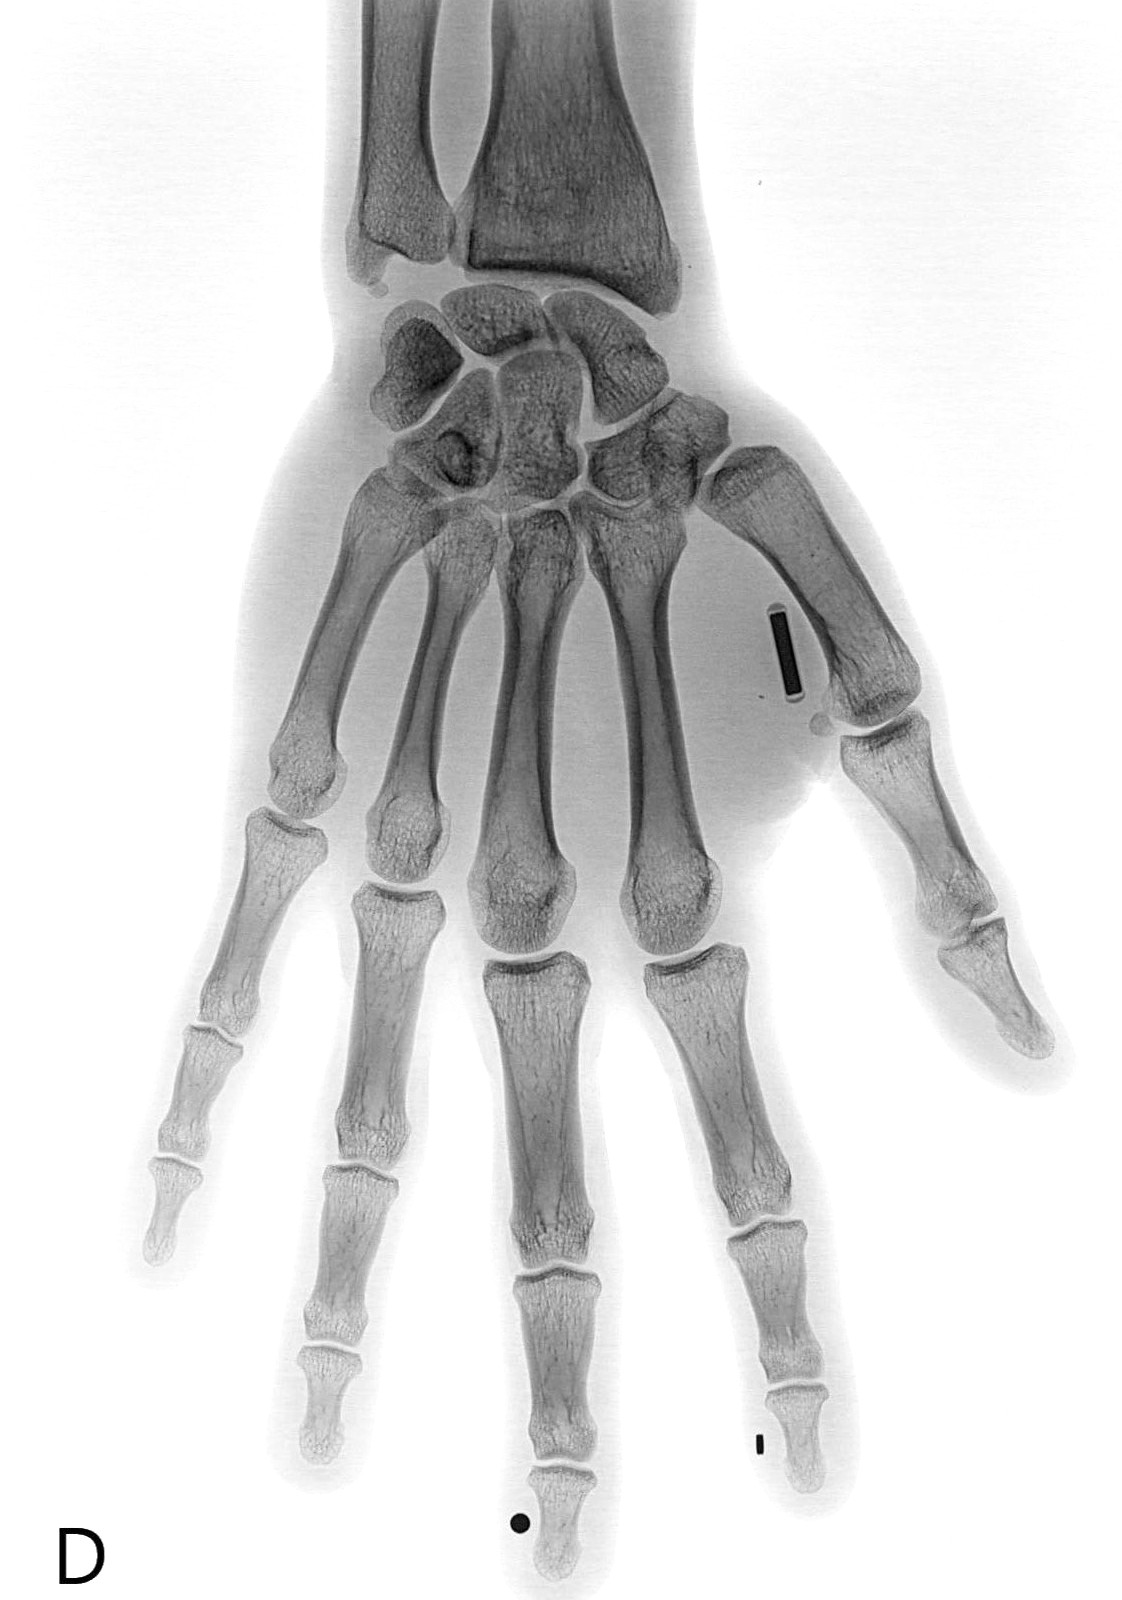
\includegraphics[width=2.5in]{FullHandXrayNeg}
				\caption{X-Ray showing the two identical finger SMIs and a larger glass-encased magnet between the thumb and the index.}
				\label{FullHandXray}
			\end{figure}
			
			\begin{figure}[!t]
				\centering
				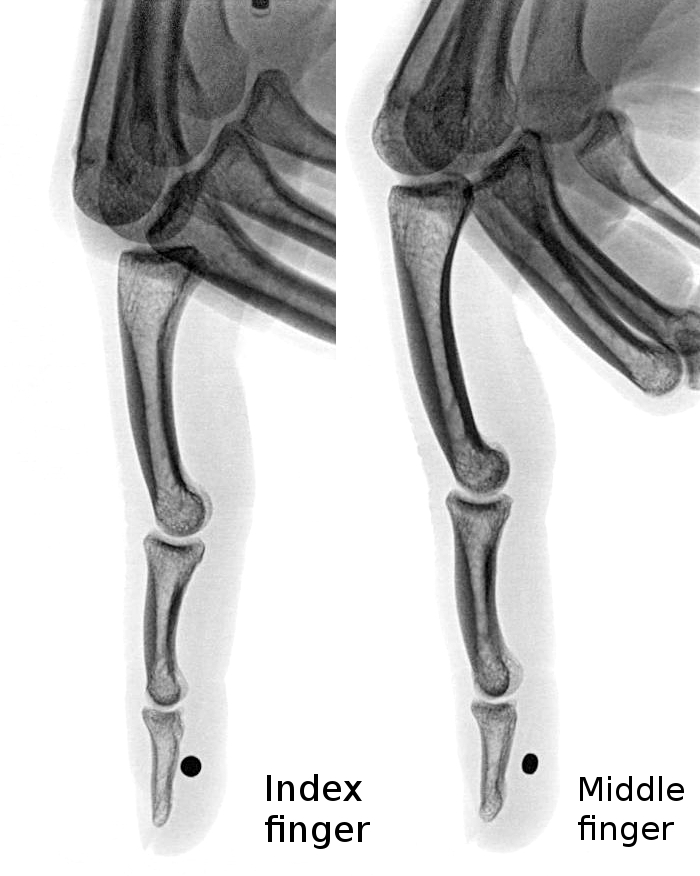
\includegraphics[width=2.5in]{FingersXrayNeg}
				\caption{Side-view X-Ray of 2 finger SMIs that have settled in different orientations.}
				\label{FingersXray}
			\end{figure}
			
%		\subsubsection{Author A. Fougues' right hand SMIs}
%		Axel's two finger implants  were implanted prior to this research (25/09/2019) for personal augmentation. As expected they provide the ability to sense magnetic fields at close proximity. For the locations, he chose the right side of the tip on his right middle and index fingers \ref{FingersXray}. These fingers were chosen for being the most intuitive way to feel something (Axel is right-handed). They are both on the right sides so that they would not stick to each other, which could become annoying on the long run.
%		
%		As clearly visible in the full hand X-Ray the two small disks have settled in a different orientation. Although they are free to rotate under a strong force it seems that they still default to this position two years later. This can be explained by the process of encapsulation, where the surrounding tissue grows back to form a capsule around the implant. This capsule having taken a specific shape can deform but will usually push the implant back to a default position.
%		Although this almost 90 degree offset in orientation has produced a very slight difference in sensitivity when sensing magnetic fields depending on their orientation, the contrast is barely noticeable.
%			
%		It is worth mentioning that a larger magnetic implant is present in the soft tissue between the thumb and the index \ref{FullHandXray}. This implant, commonly referred to as xG3, is a 15mm by 3mm Neodymium rod axially magnetized within a glass capsule. Due to its increased mass and friction it requires much stronger fields to be moved and the location is not ideal for sensing. So we won't be focusing on this one even though it might be stimulated too as a byproduct. It would nevertheless be interesting to consider it's properties in further research as its shape and mass should respond better to lower frequencies.
			
\subsection{Artificially stimulating an SMI}
Stimulation is done by creating a magnetic field around the implant. For this we use one or more electromagnets. It is then possible to vary the following parameters in order to vary the feedback:
	
	\begin{itemize}
		\item The strength or amplitude of the signal.
		\item The type of signal: sine, square, audio...
		\item The frequency, for periodic signals.
		\item The field's shape.
	\end{itemize}
	
These variations allow information to be communicated to the user through the signal. The information can be spatial because the magnetic field is continuous in space and the user can touch it and explore its shape.

Due to the nature of this process, there are in theory two ways of transmitting information by a magnetic field to an SMI:

In a first case, the field is fixed. For three-dimensional information, its shape is manipulated to reflect the information. For example a magnetic field in the form of a virtual object is projected into space and the user is free to touch it.
For non-three-dimensional information, it suffices to make the field uniform and to vary the signal according to the information. For example for Morse code the signal varies between two frequencies and can be felt uniformly throughout the space.
The works of Q. Zhang, H. Dong and A. El Saddik \cite{zhang2016ieee} come close to this technique. In their version a virtual surface is created by an array of electromagnets and can be explored using a glove with magnets on it. However, this example is based on a continuous field and the repellent effect of on the glove. A comparable version for SMIs would rely on alternating fields and the ability of SMIs to detect them even at low intensity.
While this option is ideal for large-scale 3D display applications, it inherits all of the issues associated with the formation of large and complex shaped magnetic fields.

In this second case, the field is fixed relative to the implant. In the case of our SMIs it can be produced by a ring or a bracelet for example. This time, to produce three-dimensional information, the position of the fingers will have to be monitored in real time in order to determine the appropriate stimuli in relation to their movement in space. This method has the disadvantage of having to equip yourself with a device. However, the shape of the field does not matter as long as it encompasses the implant and there can be full control of each individual implant at all times. In addition, the magnetic field to be produced is of much smaller scale, which makes the material much easier to design. In a way this is similar to the uniform fixed field but with the advantage of individual control of the implants.

We therefore opted for the second option for the control it offers and the simplicity of its design. However, our conclusions may apply in both cases.

%[THIS IS A REPETITION OF THE BACKGROUND]	
%\subsection{Sensitivity and frequency range}
%	
%In this first article on the subject of magnetic implants \cite{hameed2010ieee} Hameed et al. establish the concept of sub-dermal magnetic implants as well as some properties such as field strength sensitivity and frequency sensitivity. Although there were only two participants in the study it effectively demonstrates the principle of stimulating an implant through an external coil and gives us an idea of the results to be expected.
%	
%In a following paper \cite{harrison2018tf} Harrison I. et al. proceed to compare these magnetic implants to surface mounted implants in tests involving amplitude detection, amplitude discrimination, frequency discrimination, temporal discrimination and temporal gap detection. They demonstrated an advantageous increase in sensitivity for SMIs and a much finer sensitivity on lower frequencies (20-50Hz). They also discovered a lessened frequency discrimination on frequencies higher than 100Hz possibly due to the overlap of sensed frequency ranges between Meissner and Pacinian corpuscles.
%	
%	A possible omission in both papers on SMIs \cite{hameed2010ieee}\cite{harrison2018tf} is the importance of the implant's design (magnet-to-coating ratio, mass and shape) for the sensitivity in higher frequencies or lower amplitudes. In both cases the magnets used are common 1mm by 3mm disk implants that are made this way due to coating procedures and cost limitations. As magnet manufacturing evolves and implantables become more common SMIs are prone to evolve too, improving their performance.
	
	
%[THIS WOULD HAVE TO BE VERIFIED WITH OTHER IMPLANTEES]
%	In fact in our tests on more modern implants we found some notable differences. The tests were done in a similar manner using a Kramer PA-240Z amplifier and a coil. A Hirst Magnetics GM07 gaussmeter was used for the magnetic flux measurements. For a reliable detection at 200Hz we measured a threshold lower than 0.005mT as opposed to about 0.03mT in \cite{harrison2018tf}. The large difference can be explained by the upgraded implants (grade N52 instead of N48 and parylene coating rather than silicone) but also by the fact that our results were measured rather than approximated. Also we could not get more precision on the threshold as we were reaching the instrument's resolution limits.
%	
%	We also were interested in sensitivity over a larger range of frequencies and signals. Again testing in similar conditions we ended up with three different sensitivity curves for a sine, square and sawtooth signal.
%	
%	\begin{figure}[!t]
%		\centering
%		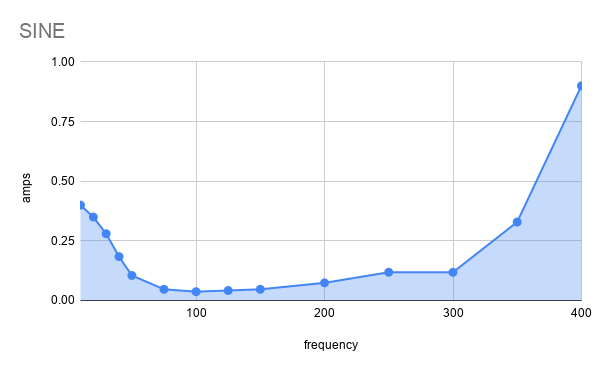
\includegraphics[width=2.5in]{SineSensitivity}
%		\caption{Relative sensitivity to a sine wave over a 10-400Hz frequency range.}
%		\label{SineSensitivity}
%	\end{figure}
%	
%	\begin{figure}[!t]
%		\centering
%		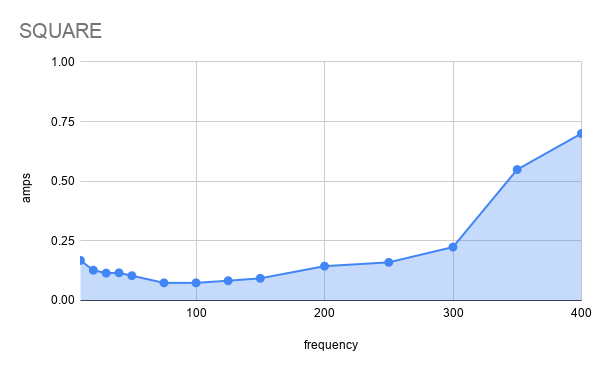
\includegraphics[width=2.5in]{SquareSensitivity}
%		\caption{Relative sensitivity to a square wave over a 10-400Hz frequency range.}
%		\label{SquareSensitivity}
%	\end{figure}
%	
%	\begin{figure}[!t]
%		\centering
%		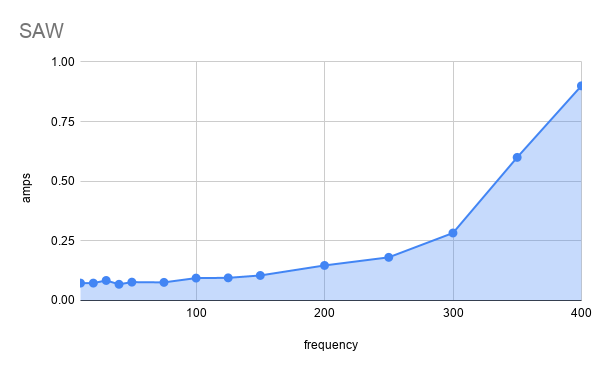
\includegraphics[width=2.5in]{SawSensitivity}
%		\caption{Relative sensitivity to a sawtooth wave over a 10-400Hz frequency range.}
%		\label{SawtoothSensitivity}
%	\end{figure}
%	
%	As you can see used current as an indicator of sensitivity. In the following estimation of the field strength $ B=\mu nI $ both $\mu$ (permeability) and n (turn density) remain constant so the current I is proportional to the field strength B. Since we can easily and accurately measure I we can therefore use it here as an indicator of sensitivity and the vertical axis is effectively the value in amps necessary to reach the threshold with an identical setup. 
%%	For this experiment both fingers were used and there was no significant difference in sensitivity between them.
%	
%	The results are visibly different for each signal. The most sensitive range overall being 50-300Hz as expected. Also all signals lose sensitivity rapidly over 300Hz.
%	On low frequencies (<100Hz) the sharp polarity changes in the square and saw waves make them stand out more while the sine wave tends to fade out. This makes sense, in lower frequencies the sharp drops in the saw wave produce a fast change in polarity that can be assimilated to a pulse signal and be felt more easily even in very low frequencies.
%	In the mid-range (100-300Hz), the sensitivity threshold is similar for all waves.
%	Above 300Hz we can see that the square wave does not fade as quickly as the other two.
%	As the frequencies get higher above 300Hz the changes in polarity become too close to be sensed. We can see that the square wave is slightly less affected. It is difficult to explain but we can suppose that the square wave (and saw to some extent) should be felt better in the higher frequencies as the changes in polarity are further apart and sharper.
%	The reason saw waves are less sensitive than square waves in high frequencies might be that the sharp polarity change is always in the same direction and contrary to low frequencies the implant does not get enough time and/or energy to move all the way back.
%	In \cite{harrison2018tf} amplitude detection was only tested on two frequencies, here we test them over a range. Nevertheless the higher sensitivity at 200Hz than 20Hz (Amplitude RL results, sine) is similar in our results.
%	
%	As tested and proven in \cite{chan2012lnecs} tactile stimuli also has the advantage of producing much faster response times than its visual and audio counterparts with no significant influence from the position of the stimuli.
%	
%	Describing the sensations produced by the stimulation is very subjective but a general idea can be given. As such we have categorized the sensations:
%	\label{categorization}
%	\begin{center}
%		\begin{tabular}{ | m{5.5em} | m{0.5em}| m{17em} | } 
%			\hline
%			Incoherent & I & Hard to recognize the signal. Noise or a continuous signal with spikes in amplitude. Like holding a bee. \\
%			\hline 
%			Continuous & C & Feels like lightly sliding the finger across smooth fabric or very soft fur. \\ 
%			\hline
%			Vibration & V & A soft vibration of discernible frequency, not very localized and fades throughout the finger. Can feel like rough fabric. \\ 
%			\hline
%			Buzz & B & A sharp vibration that reverberates through the bone. A pull on the magnet's area can be felt at the same time. Feels like touching a running engine or running your fingers against the bars of a fence. \\ 
%			\hline
%			Tapping & T & A sensation of being hit or tapped at the implant's location at a speed equivalent to the frequency used. \\ 
%			\hline
%			Deformation & D & Feels like something is crawling under the skin, similar to rubbing the finger on a surface of small beads 
%			or pressing on a small ball bearing. \\ 
%			\hline
%			Pull & P & Very localized feeling of the implant being attracted in a direction (the direction can be hard to determine). It is a continuous version of "Tapping" but the mechanoreceptors get used to it so quickly that it takes a lot of power to be felt reliably. \\ 
%			\hline
%		\end{tabular}
%	\end{center}
%	
%	The order they are in loosely correlates to the frequencies they correspond to with very high frequencies tending towards I and low ones towards P but over all different signals tend to intensify different sensations.
%	For example a sawtooth wave will produce a very distinct T while a sine will be much closer to a D.
%	It is also important to mention that depending on both signal type and frequency each of these sensations can feel sharper or smoother while still belonging to the same category. Effectively making it possible to differentiate one signal type from another even though the produced sensations are similarly named. 

%[IS THIS PART NECESSARY?]
%	\subsection{SMI key benefits and drawbacks for haptic rendering}
%	By comparing to existing methods we can deduce the strengths and flaws of our implant-based technique. Of course we take into account the constraint of having to have one or more implants placed. However, in view of the trends \cite{duarte2014ne} and the potential of body hacking we will remain optimistic about a future where (non-medical) implants are widespread and accepted.
%	
%
%	Benefits:
%	
%	\begin{itemize}
%		\item As with the ultrasound method, our technique does not require direct physical contact to the stimulated area of skin.
%		\item Our method allows higher and finer force feedback (as opposed to the weaker ultrasound feedback).
%		\item The system is mechanically simple and therefore compact, versatile and scale-able.
%		\item Magnetic fields are unobstructed by the vast majority of bodies and materials (again as opposed to ultrasound). They are also not noticeable by humans and the majority of living beings.
%	\end{itemize}
%	
%	Drawbacks:
%	
%	\begin{itemize}
%		\item SMIs only stimulate at one point (each), therefore we do not have the resolution of a mechanical system or the ability to cover an area like the ultrasound-based system.
%		\item The range of a magnetic field is limited. A magnetic field follows the inverse cube law ($ R ^ {- 3} $). This can be compensated to a certain extent by a more powerful system.
%	\end{itemize}
	
\section{Wearable stimulator design}
In order to be able to experiment with our ideas, we had to create the device that will transform our signal into a magnetic field. For this we have considered many options, including a device in the form of a bracelet. This bracelet could consist of a single large electromagnet encompassing all the implants of the hand in a single field or of a set of electromagnets arranged in a circle. This second option would theoretically have allowed the creation of complex shaped fields, essentially forming a "magnetic display" (similar to that of Q. Zhang \cite{zhang2016ieee}) around the hand.

The alternative considered was that of rings whose body constitutes the electromagnet. In order to test all these different configurations and the ways to optimize the magnetic flux, we used simulations. We used a finite element analysis software (Finite Element Method Magnetics). Unfortunately, obtaining the sufficient field range for this application would have required the manufacture of complex custom-made coils with metal cores and the final format did not necessarily meet our criteria.

Finally we have chosen a new system in the form of rings using an unshielded axial inductor to produce the signal. The support rings are modeled and printed in PLA \ref{PLARings}.

	
	\begin{figure}[!t]
		\centering
		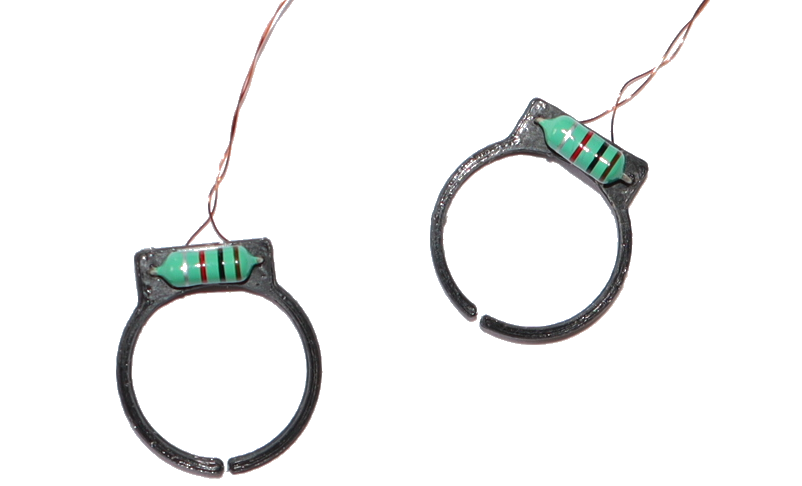
\includegraphics[width=2.5in]{PLARings}
		\caption{A ring design utilizing a single axial inductor on a 3D printed base.}
		\label{PLARings}
	\end{figure}	
	
	\begin{figure}[!t]
		\centering
		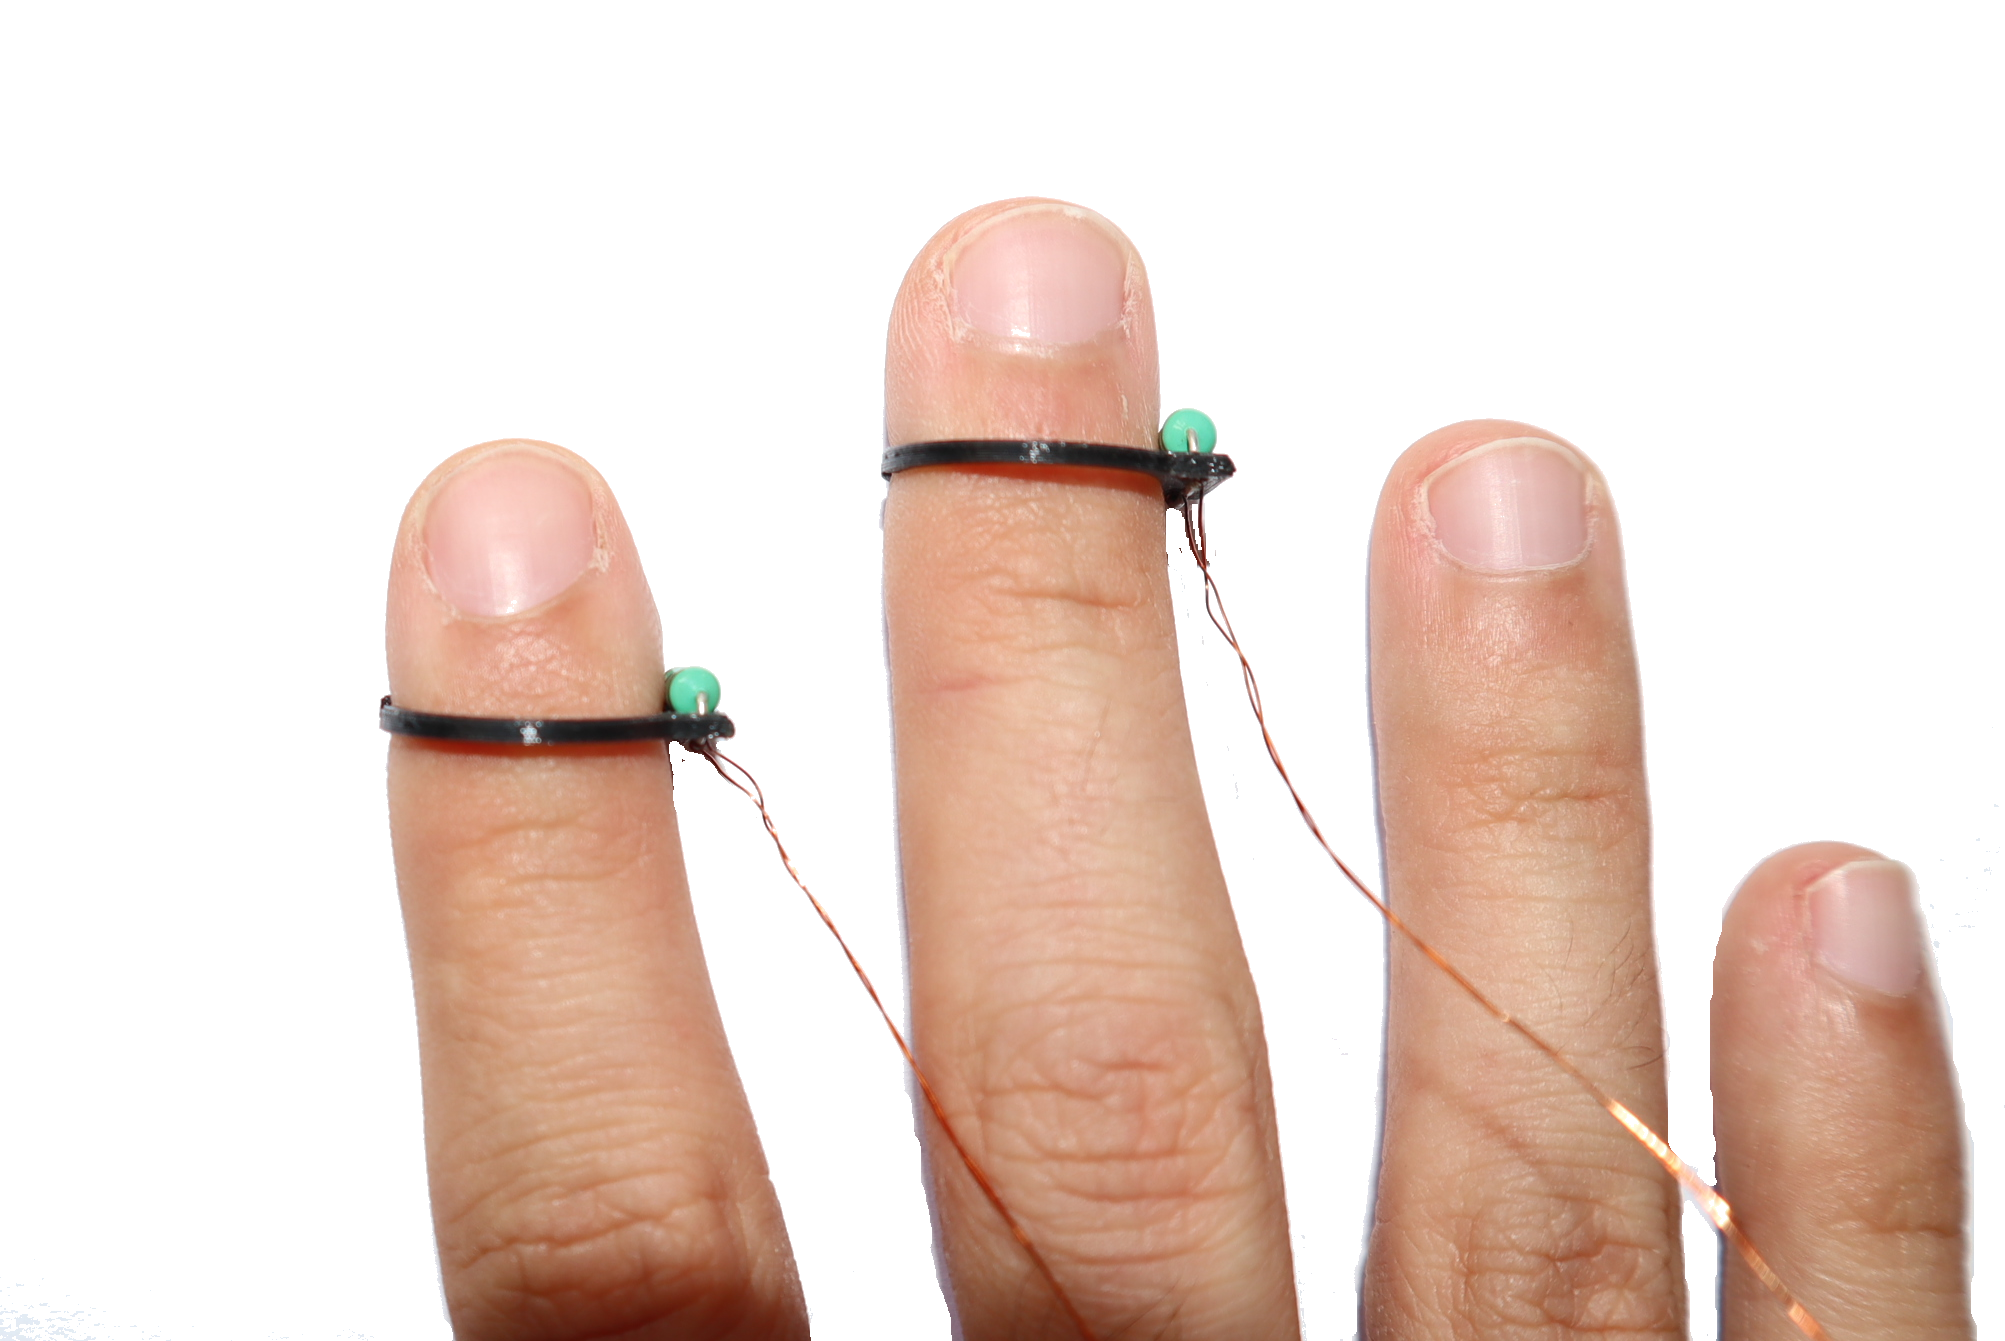
\includegraphics[width=2.5in]{FingersWithRings}
		\caption{Ring worn at close proximity to the implant.}
		\label{FingersWithRings}
\end{figure}

Given the desired frequency and intensity range we have decided to treat our signals as standard audio. The disadvantage of this method is that the production of frequencies below 50Hz is often limited by the hardware. However, it offers the advantage of being able to use the existing protocols and audio channels of our devices (bluetooth, aux outputs, etc.).

The rings are therefore connected to the outputs of a portable audio amplifier. Initially we considered the use of custom rolled coils however the use of inductors proved to be more compact and more coherent while the loss in performance is negligible. Due to their small size and the nature of the inductor used, bands must be worn at implant level \ref{FingersWithRings}.

The inductor is chosen such that its resistance limits the maximum current that can be produced by the amplifier so that it corresponds to the maximum current supported by the inductor. In this way no additional components are needed and the inductor is used to its full potential. We can of course use the two stereo channels to control two rings separately. For our rings, a 5W two-channel amplifier proved to be sufficient. Therefore the amplifier is only a few centimeters. We use power cable and audio-jack cable for signal input. The rings are connected to the outputs of the amplifier by very fine wires of about 1 meter. 

This system meets our main criteria:
\begin {itemize}
\item At least two fingers can be stimulated independently.
\item The fabrication is easy and the performance of each ring is consistent.
\item The device is discreet and is not restraining the user.
\end {itemize}

A wireless version with a Bluetooth amplifier and a small on-board battery was also made \ref{HandBluetooth} but the delay introduced by the Bluetooth protocol was deemed too important.
A held version with a finished design in a solid PLA enclosure was made in parallel \ref{SMISCUBE}. Although not usable for AR and VR it was very convenient for testing and can be used in many other use-cases some of which are mentioned in the conclusion of this paper [FUTURE REF HERE].

\begin{figure}[!t]
		\centering
		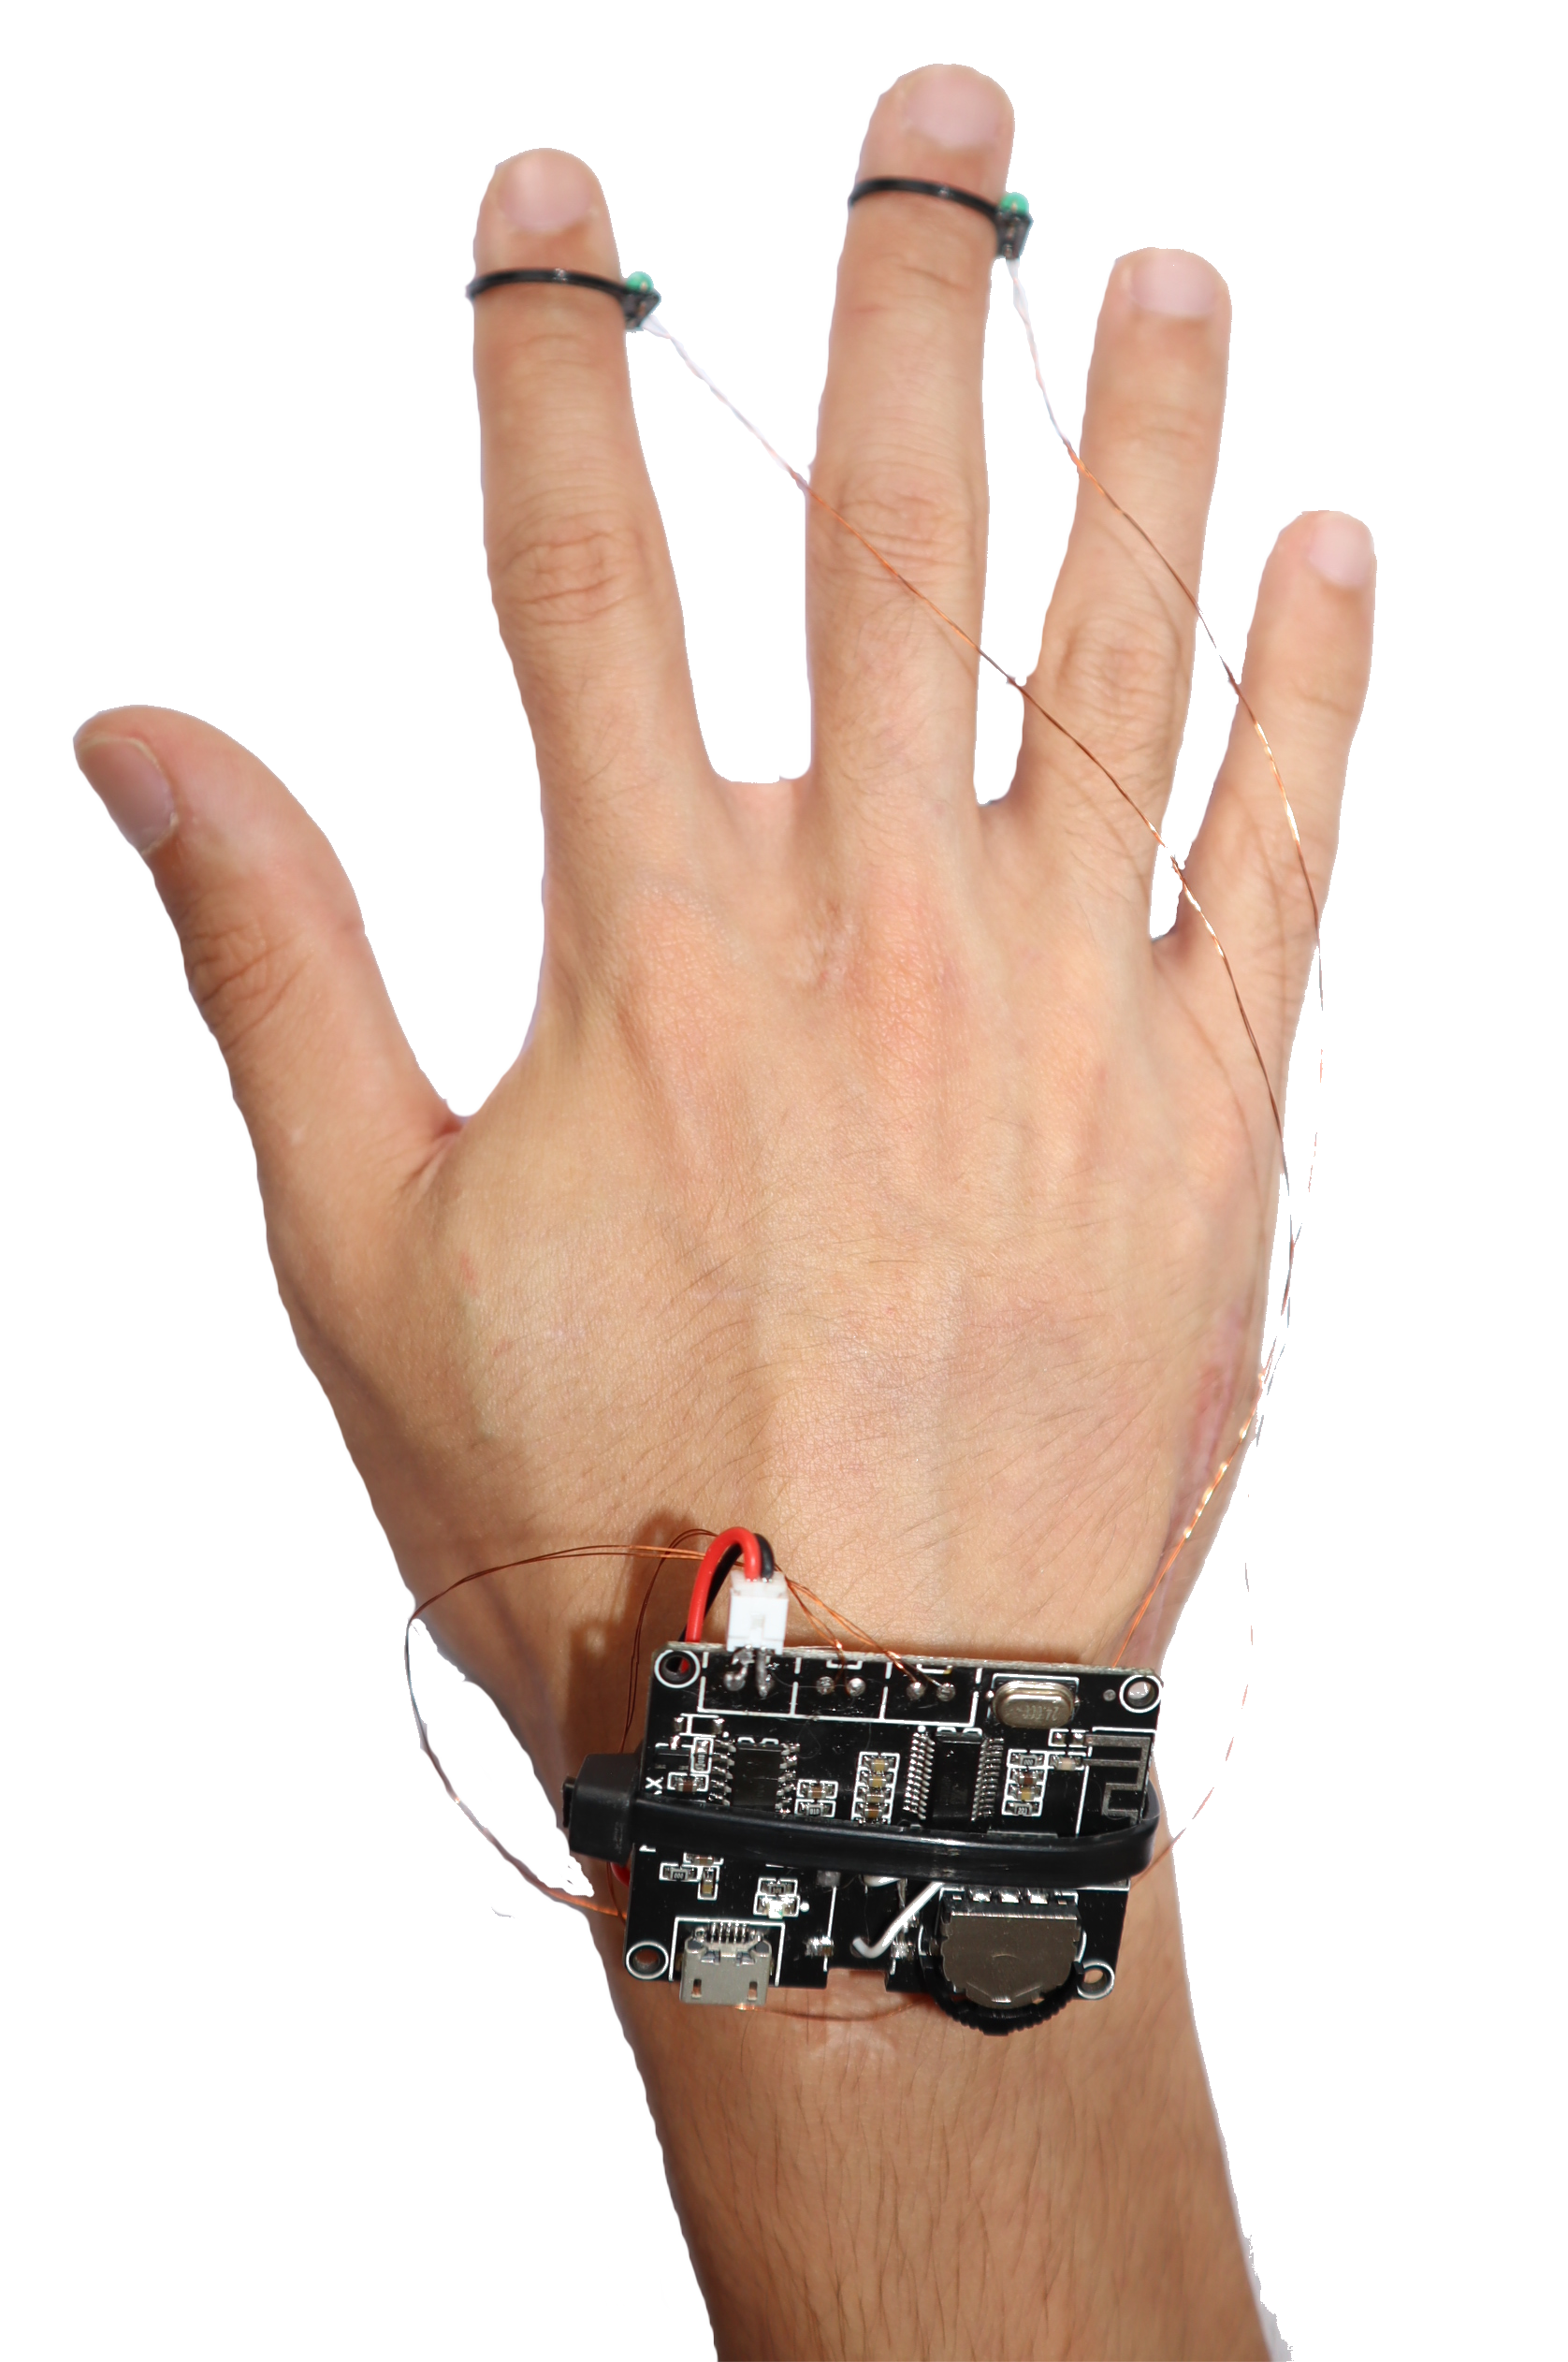
\includegraphics[width=2.5in]{HandBluetooth}
		\caption{Ring worn at close proximity to the implant.}
		\label{HandBluetooth}
\end{figure}

\begin{figure}[!t]
		\centering
		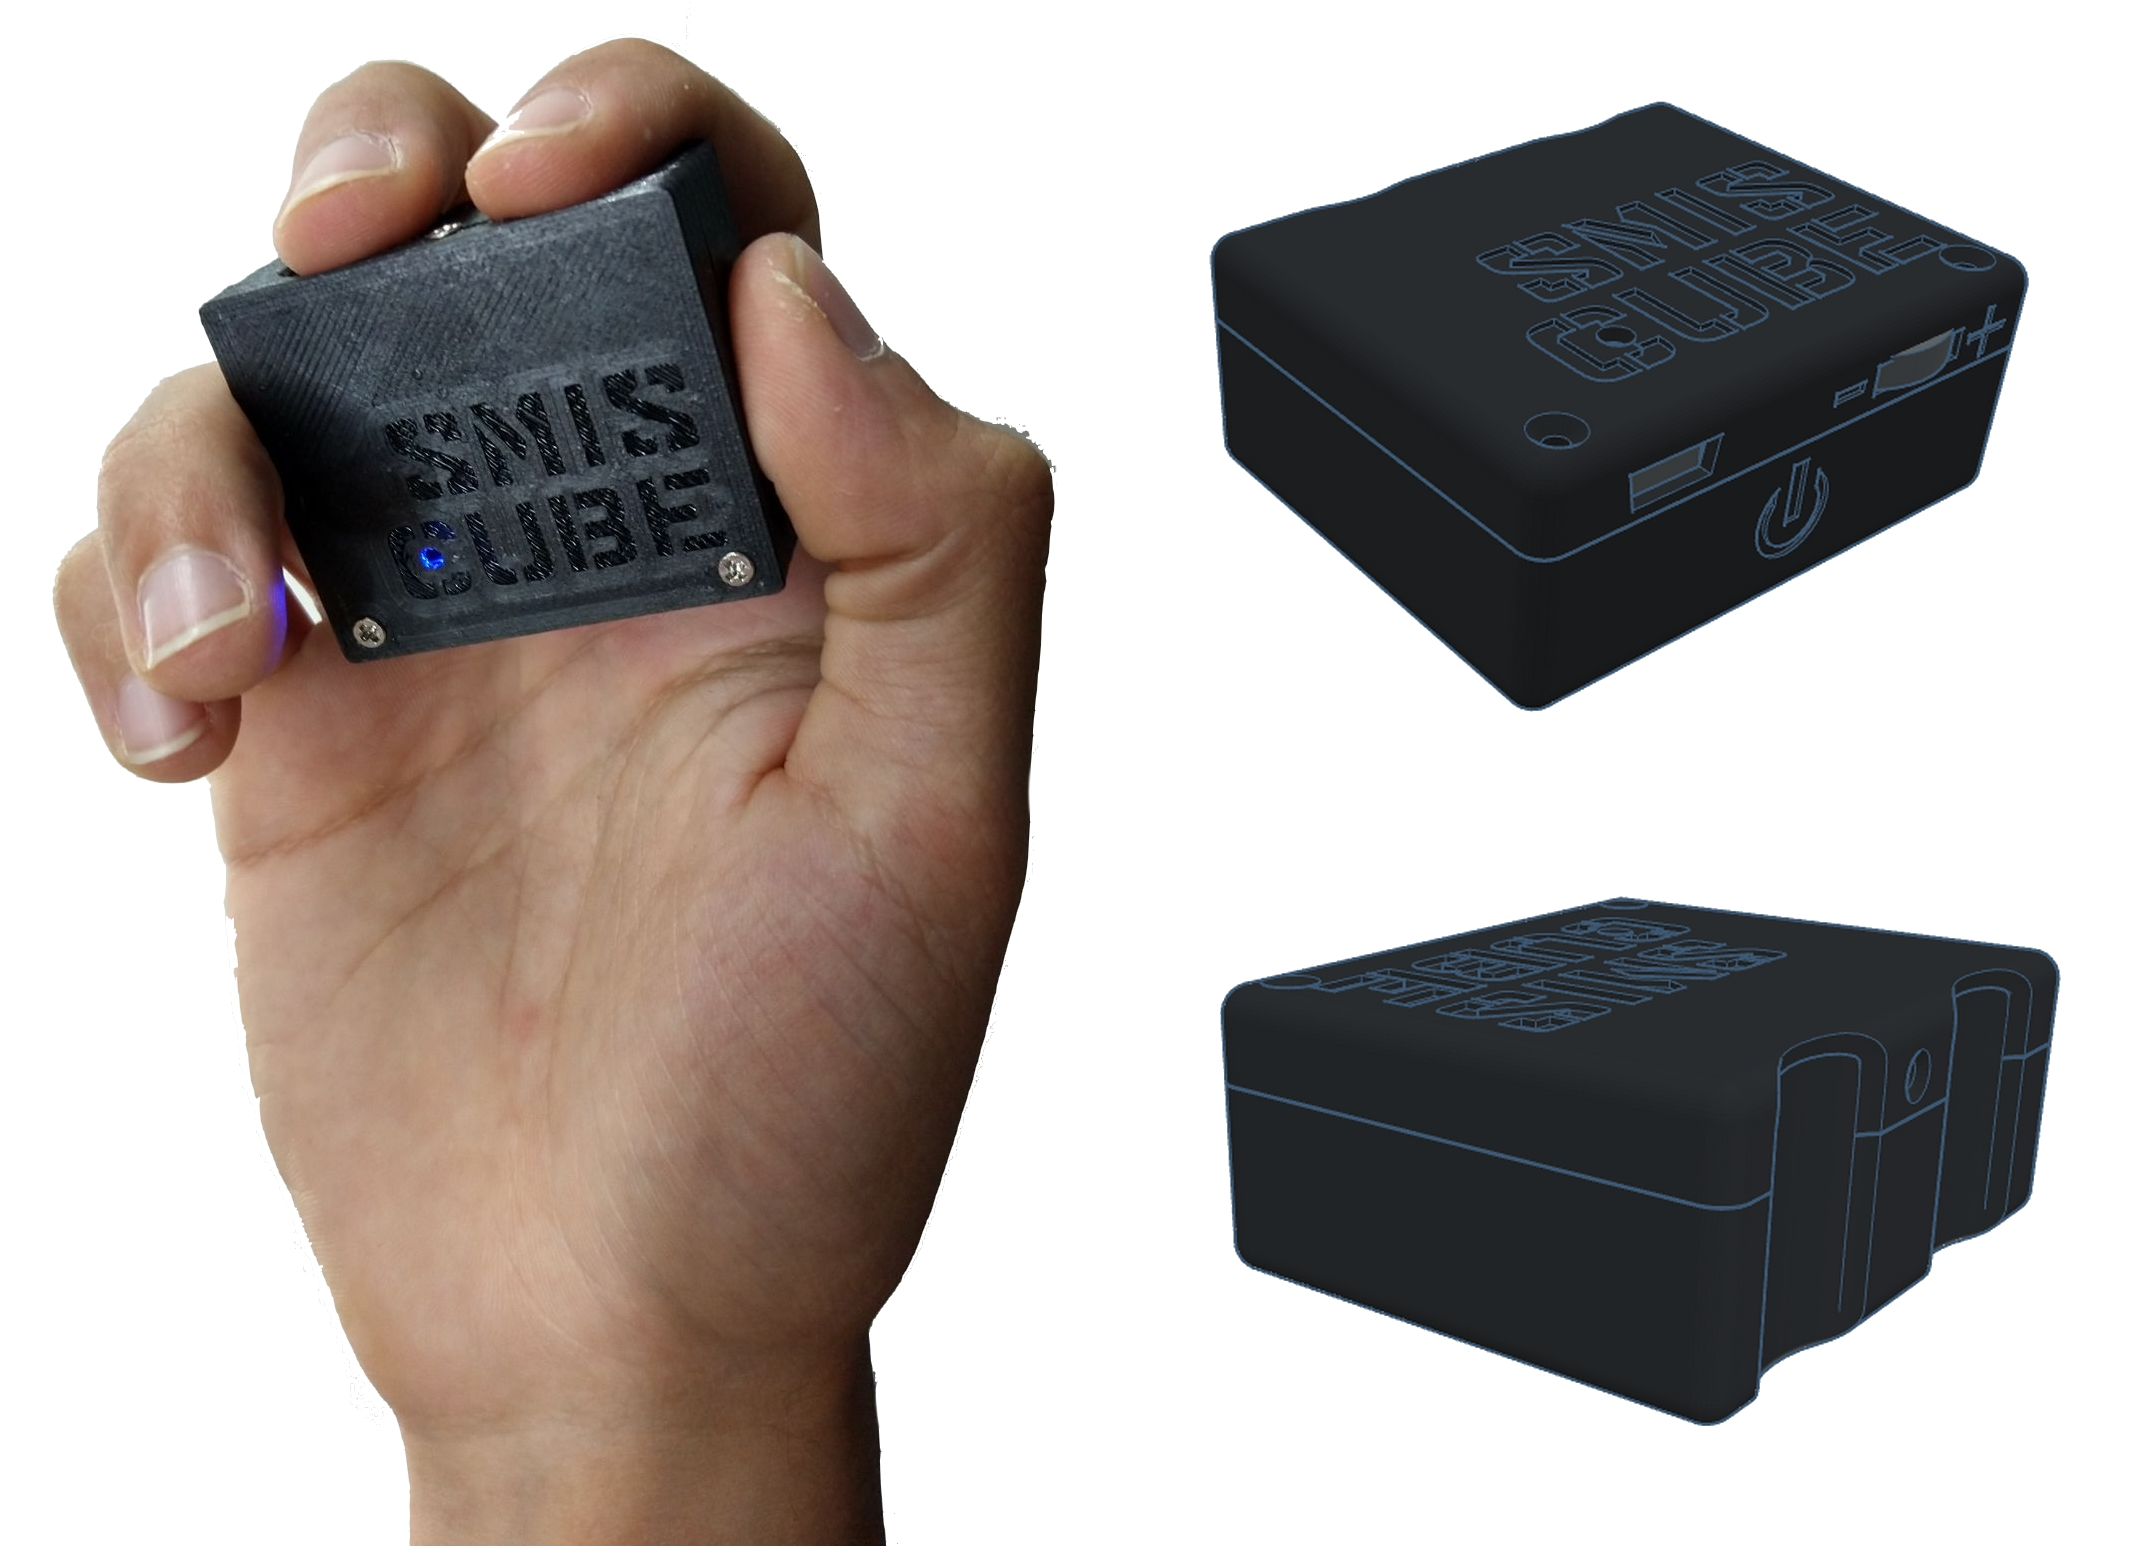
\includegraphics[width=2.5in]{SMISCUBE}
		\caption{Ring worn at close proximity to the implant.}
		\label{SMISCUBE}
\end{figure}

\section{Haptic rendering of a virtual environment}
	Based on the limitations and advantages of this method here is an overview of potential use-cases at the moment divided into three categories. We propose to use SMIs as a haptic feedback device in virtual environments, augmented reality and robot control. They would provide pressure and texture feedback while retaining an extremely low mechanical complexity and low constraint for the user. We will be using Unity to construct a virtual scene and a LeapMotion to keep track of the user's hands within this scene. The previously designed device will produce a feedback corresponding to the hand's (more specifically the fingertip) overlap and movement relative virtual objects.
	
\subsection{Pressure/collision feedback}
From the 3D virtual interaction we first extract the depth of penetration of the fingertip in the object perpendicularly to the closest object surface point. This value will directly correlate to the felt pressure. The pressure will be defining the amplitude of the feedback signal.
 
In this simple scenario the signal is sine-wave of low frequency (around 50 Hz)for a finer amplitude discrimination \cite{harrison2018tf}. 

Every material has a "surface thickness" that defines the depth at which maximum amplitude is reached: It is composed of two depth buffers. 

The first one is very shallow and can be assimilated to the softness of the fingertip. It creates a slight transition between no stimuli and maximum stimuli that is closer to realistic expectations of pressing against even the hardest material. Therefore this buffer is fixed at X mm and common to all solid materials.

An additional value can be added to represent the object's softness. This one can be adjusted for each material type and simulates, in a simplistic but sufficient way, the give of the surface when under pressure from the fingertip.

The evolution of pressure along this combined depth can left linear or adjusted in the form of a curve to produce more convincing feedback. Ease-in curves can for example be more convincing in very soft materials as the tend to replicate the non-linear "elasticity" of the material.

\begin{figure}[!t]
		\centering
		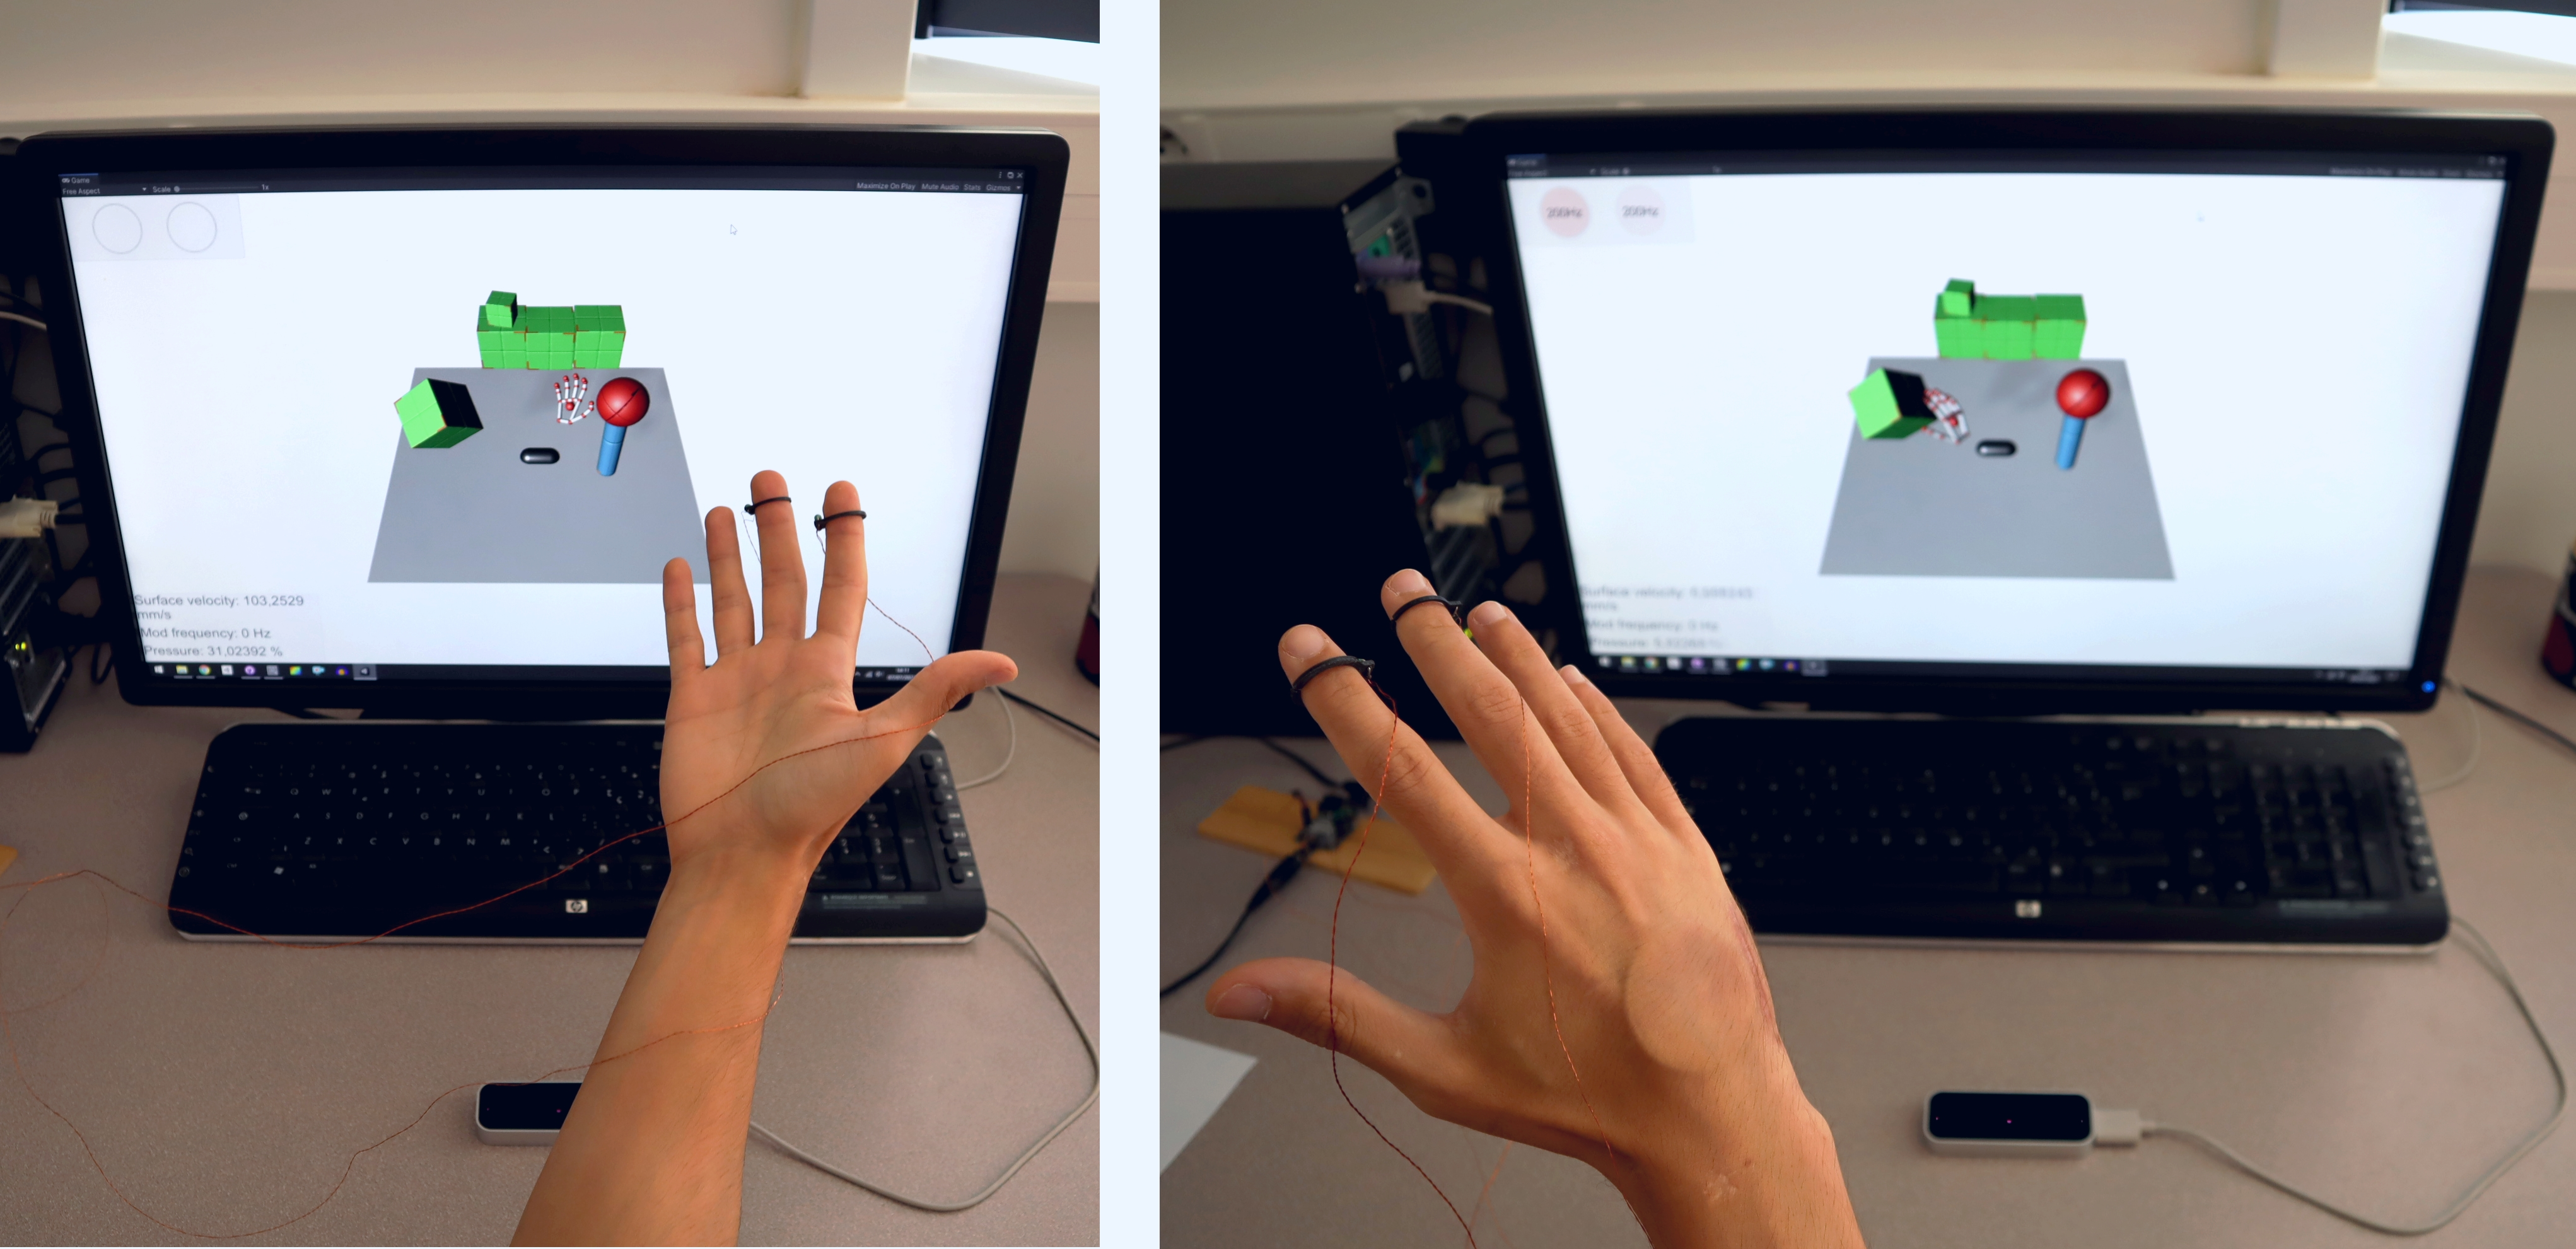
\includegraphics[width=3.5in]{Setup}
		\caption{Ring worn at close proximity to the implant.}
		\label{Setup}
\end{figure}
%	We were able to verify this simple implementation by using it with simple shapes (cubes and spheres) and no visual feedback. Just by reaching around in space and following the contour of the shapes with the fingertips it was easy to get a mental picture of the scene.
\subsection{Texture rendering}
	Then we try simulating texture. For that we assign each material a spatial period representing the coarseness of it's texture. We then calculate the tangential velocity of the fingertip to the object's surface and with the following formula \cite{bensmaia2003smr} we deduce the feedback frequency:
	$F = tangential velocity / spatial period$
	This frequency can the be applied as an amplitude modulation on our previously described signal or can directly replace the 50Hz base frequency.
	Sadly the calculation of the tracked finger's velocity introduces a lot of unwanted noise as opposed to the simple collision tracking used for the pressure simulation. This is of course due to the tracking precision of the LeapMotion controller but also to the natural shaking of a hand in empty space (the shaking would not be present when touching an actual physical object due to friction). In the optimal lighting condition for the hand tracking and by filtering the values with a rolling average we still get spikes in absolute velocity of up to 6 mm/s. This can be reduced by further filtering but then the input delay becomes noticeable.
	This means we can either threshold the texture simulation to a minimum velocity which gives inconsistent feedback on slow movements or the feedback can be left as is but the feedback for a static touch will remain noisy. We found the second option much more distracting. 

\subsection{Recognizable prerecorded transient feedback}
Regarding haptic rendering in a virtual environment there is one last interesting point to explore. These are punctual and very recognizable daily haptic feedback. In particular the physical "click" of a mechanical button or a switch. We chose this example because it is intuitive and how it feels can vary from button to button.
After considering producing the stimuli procedurally, we realized that in the majority of cases the audio produced by the button is very similar to the physical feeling of the button. So we tried to use audio recordings directly as stimuli. The result is very good and gives a feeling very close to the real experience.
In some cases it can be interesting to shift the frequencies of the audio track towards the sensitive range of the implants.
[More details here]
	
\section{Haptic rendering of alternative sources}
	When considered as less disrupting alternative to visual (screens) or audio(speakers) input SMIs can be envisioned as a new discrete information streaming route from digital devices to the brain. 
	In this first idea the device could be connected to sensors of any type effectively creating what is referred as sensory substitution. A common example is using an ultrasound range finder to aid in the navigation of blind people. In this example a feedback is given relative to the distance of the person to an obstacle. In a similar way a microphone can be used for the deaf. 
	This last example has been tested extensively using surface of the skin vibration with very conclusive results. With training participants were capable to recognize and differentiate sounds in \cite{perrotta2021neuroscience}. This is good evidence that similar results if not better could be achieved with SMIs. The interesting lead on this option is to think of all the possible "artificial senses" one could learn. The "North Sense" trans-dermal implant is also a great example of what can be done through sensory substitution. Created and used by Liviu Babitz, it constantly notifies the user of their orientation through a vibration on the chest. Over time users have reported being intuitively aware of their geographical orientation without consciously paying attention to the implant.
%	\paragraph{Media and digital sense}
%	We spend hours interacting with the digital world and that interaction usually fully engages at least on of our main senses making it difficult or impossible to execute another task at the same time. We would like to use our auxilary information channel to free the user's hands, ears and eyes while still streaming information to them.
%	On the most basic level, for example, the device is connected to a users phone and relays notifications and ringing through the SMIs. On a much more advanced level, complex information (sound, speech, directions) could be streamed to the user continuously without impeding them of full sensory capacity (hearing, looking, touching) and mobility (using their hands) like holding a phone would.
%	This concept can be difficult to imagine but basing ourselves on existing research on sensory substitution through touch and concepts like brain plasticity it should be possible to an extent.
	
\section{Experiments}
The experiments on haptic rendering will be done using Unity combined with a Leapmotion controller placed flat on the desk in front of the user. For the stimulation the device detailed earlier will be used.

\subsection{Shape recognition and scale}
\subsubsection{Material and methods}
\label{Shape recognition and scale}

We want to test how effective the 3D feedback is at giving the user information about the virtual objects he is touching. For that we will be asking the subject to discriminate between three simple 3D shapes by touch alone. We will be varying the scales of the objects at each round.

This is how we will proceed:
The test subject will be equipped with our stimulation device. Ideally two rings will be used on two implants unless the subject only has one in which case only one will be used. The subject will be seated at an empty desk with just the Leapmotion controller in front of them. 

At each turn three shapes (a sphere, a cube and a cylinder?) will be presented to the subject. Their scale will be randomly selected (uniform for the three shapes). The subject will be given time to touch them and try to tell which is which. The experiment will be repeated with a variety of scales.

This experiment will hopefully give as clues as to the effectiveness of the feedback in 3D while taking into consideration the limitations in spatial accuracy that the hardware and software could give rise (by keeping track of the scale).
We will of course be monitoring the answers to the test in relation to the scale but we will also be logging the finger trajectories that could be interesting to analyze thereafter.

\subsubsection{Results}
		
\subsubsection{Discussion}

\subsection{Hardness/force discrimination}
\subsubsection{Material and methods}

In testing hardness we wish to determine if the simulation of different material properties can effectively be rendered through the SMIs.

In this effect three cubes will be presented in a similar fashion to the previous experiment \ref{Shape recognition and scale} except this time the subject will have a visual representation of the cubes and his hand(s) on a screen as this should not impact the experiment and helps with finding the objects. The cubes will be visually identical.

At each turn, a randomized hardness will be attributed to each cube (different for each). The subject will be asked to rank them (from softer to harder) by touch.

With this experiment we hope to demonstrate the variability of pressure feedback and hopefully determine a discrimination threshold. If possible we will also use non-linear feedback curves [Need to find papers on the subject]

\subsubsection{Results}
		
\subsubsection{Discussion}

\subsection{Effectiveness of punctual recognizable feedback}
\subsubsection{Material and methods}

The simplest stimulation we can produce in a virtual environment is a simple short pre-recorded signal, yet it might be hugely effective, especially if it is a tactile response that the user is familiar with.
We want to determine the effect of such a feedback on the precision and dexterity increase of a user when the feedback expected from real world circumstances is produced through the SMIs.

To do so we take the example of a simple and familiar mechanical button click. The subject will be seated in front of a screen and the Leapmotion controller. On the screen will be represented the virtual environment consisting of an array of five large buttons on a wall facing the user and a representation of the user's hand in that space. Each of the buttons has a corresponding light over it. The buttons are animated and can be "pressed" by the user. At each turn the buttons will be producing a feedback or won't. We will then ask the subject to quickly turn all the lights on.

We expect the absence of a feedback to confuse the user into pressing the buttons too much or too little effectively loosing time. We hope that the familiar response of a button clicking when sufficiently pressed will allow for the task to be done more cleanly and quickly. We will be tracking the fingers to analyze the depth and consistency of the presses.
[I would like to find 1 or 2 other examples than buttons]


\subsubsection{Results}
		
\subsubsection{Discussion}

%%Shape recognition
%[Not sure how the results of this one can be used?]
%The first experiment will aim at determining the extent of virtual 3D shape recognition using only the haptic feedback of SMIs. To do so the test subject will be equipped with our device. Ideally two rings will be used on two implants unless the subject only has one in which case only one will be used. The subject will be seated at an empty desk with just the Leapmotion controller in front of them. They will be told that there is a shape in front of them at eye level and will be given time to touch the shape until they are ready to make a guess as to what shape is presented. No visual feedback will be given. The feedback provided during the experiment will be the pressure feedback with no texture of a randomly selected shape. The shape will have overall dimensions under 30 cm in the real world so as to fit within the Leapmotion's field of view and be easily within reach of the subject.
%We can use simple solids that are easy to describe: cube, sphere, pyramid, cylinder.
%

%[Again what will the results be compared to? What can we conclude after doing this?]
%In a second experiment we use a similar setup. In the space in front of the subject will be a virtual path formed of straight segments going from the left to the right with a random amount of corners (0 to 5). The subject is asked to follow the line from the left to the right while counting the number of corners. This can be repeated while reducing the angle of the bends which should make the counting harder or the thickness of the path to make the following harder. We will be monitoring the answers as well as the followed trajectory.
%

%[This one mixes force feedback and "click" feedback, they should be treated separately]
%%Caracteristic feedback recognition
%In this last experiment we wish to prove the subject's ability to discriminate between the force feedback of multiple different virtual buttons.
%The subject will be seated in front of a screen and the Leapmotion controller.
%On the screen will be represented the virtual environment consisting of an array of five large buttons on a wall facing the user and a representation of the user's hand in that space. The buttons are animated and can be "pressed" by the user. A randomized "hardness" will be attributed to each button. The subject will then be asked to press the buttons and rank them in order of felt hardness using the stimulation device.

%[Additional things I would like to test that do not necessarilly belong here:]
\subsection{Evolution of sensitivity thresholds}
\subsubsection{Material and methods}
It would be interesting to test the lowest detectable amplitude of a 200Hz sine so that we can compare the results with \cite{harrison2018tf} I. Harrison's and therefore know if changes in design of the implant in the last years make a significant difference in sensitivity. To do so we would use a fixed coil of similar dimensions as in \cite{harrison2018tf} Harrison's paper. On the bottom center of the coil we place a gaussmeter probe and we also monitor the drawn current. The subject then places their finger in the center of the coil and either no signal or a signal of randomized amplitude is sent through the coil. Each time the subject says if the stimuli was felt.
We expect lowest thresholds around 0.005 mT instead of the 0.03 mT average found previously. Also the gaussmeter will allow us to validate the estimated field strength as we expect that there is a significant difference between estimated and measured values.

Additionally the previous experiment could be repeated with varying frequencies for a sine, square and sawtooth wave to obtain sensitivity curves for each \ref{SineSensitivity} in a more reliable way. This might take some time though as there is 42 frequency-signal type configurations to be tested.

Finally we could validate my categorization of sensations \ref{categorization} by giving a series of stimuli to the subject and asking them to assign a category to each. If the results match between subjects then the description can be considered as accurate.

\subsubsection{Results}
		
\subsubsection{Discussion}

\subsection{Alternative feedback sources}
\subsubsection{Material and methods}
For this second set of experiments we wish to test the understanding of basic information when transmitted through SMIs.

%This will test the understanding of continuous information as expected from most environmental sensors
Firstly we would like to experiment with the transfer of continuous information such as provided by most environmental sensors. We will use the on-board compass of the android device to keep the subject aware of their current cardinal orientation. We hope that the subject will be capable of keeping track of their orientation independently of visual cues and memory. To test this the subject will be equipped with the android device in a frontal or rear pocket making sure that it will be held firmly against the body and not rotate relative to the body. They will then be equipped with the stimulating device and blindfolded. The subject is told to memorize their orientation. We finally proceed to spin the subject around and ask them to face back to their original orientation. This will be repeated five times without any stimuli and five times with it.

[I would like to add a second navigation-related experiment here...]
		
\subsubsection{Results}
		
\subsubsection{Discussion}
		
\subsection{Further research}

\subsubsection{Long term sensory substitution}
We're interested in exploring the extents of sensory substitution through this new medium. An idea would be to use audio signal of sound or speech to the stimulate the implants. To get the best results the signal would have to be remapped in the frequency domain from it's original range to something close to our tactile sensitivity. Of course remapping the full audible spectrum (20-20,000Hz) to our limited sensitivity of 10-300Hz would lead to an extreme loss of resolution but simple sounds such as speech use a much more reasonable range. Hopefully, through extensive training, simple sounds or speech could be understood. 
Alternatively method's like the ones used in the Neosensory Buzz \cite{perrotta2021neuroscience} might be applied.
If it ever turns out that such complex information can be interpreted through this medium it's design simplicity and convenience will shine in many fields like helping with disabilities, discreet communication, information streaming in high stress scenarios \cite{harrison2014thesis} and of course augmented reality.
\subsubsection{Shaping the magnetic field}
An other lead that we hinted at earlier is the use of this technology on much larger scales. Assuming it is possible to produce fully controllable room-sized magnetic fields then a user within that space could be provided with information while being completely free of any equipment. This could in theory be used to render full scale tactile virtual environments, establish silent and targeted communication or even 3D guidance. An obvious use for that would be in VR entertainment but it could also be used in dangerous or high stress workplaces.
Of course the use of SMIs in such a large scale depends largely on our ability to produce and manipulate magnetic fields which is an ongoing filed of research to this day. 

% needed in second column of first page if using \IEEEpubid
%\IEEEpubidadjcol




% An example of a floating figure using the graphicx package.
% Note that \label must occur AFTER (or within) \caption.
% For figures, \caption should occur after the \includegraphics.
% Note that IEEEtran v1.7 and later has special internal code that
% is designed to preserve the operation of \label within \caption
% even when the captionsoff option is in effect. However, because
% of issues like this, it may be the safest practice to put all your
% \label just after \caption rather than within \caption{}.
%
% Reminder: the "draftcls" or "draftclsnofoot", not "draft", class
% option should be used if it is desired that the figures are to be
% displayed while in draft mode.
%
%\begin{figure}[!t]
%\centering
%\includegraphics[width=2.5in]{myfigure}
% where an .eps filename suffix will be assumed under latex, 
% and a .pdf suffix will be assumed for pdflatex; or what has been declared
% via \DeclareGraphicsExtensions.
%\caption{Simulation results for the network.}
%\label{fig_sim}
%\end{figure}

% Note that the IEEE typically puts floats only at the top, even when this
% results in a large percentage of a column being occupied by floats.
% However, the Computer Society has been known to put floats at the bottom.


% An example of a double column floating figure using two subfigures.
% (The subfig.sty package must be loaded for this to work.)
% The subfigure \label commands are set within each subfloat command,
% and the \label for the overall figure must come after \caption.
% \hfil is used as a separator to get equal spacing.
% Watch out that the combined width of all the subfigures on a 
% line do not exceed the text width or a line break will occur.
%
%\begin{figure*}[!t]
%\centering
%\subfloat[Case I]{\includegraphics[width=2.5in]{box}%
%\label{fig_first_case}}
%\hfil
%\subfloat[Case II]{\includegraphics[width=2.5in]{box}%
%\label{fig_second_case}}
%\caption{Simulation results for the network.}
%\label{fig_sim}
%\end{figure*}
%
% Note that often IEEE papers with subfigures do not employ subfigure
% captions (using the optional argument to \subfloat[]), but instead will
% reference/describe all of them (a), (b), etc., within the main caption.
% Be aware that for subfig.sty to generate the (a), (b), etc., subfigure
% labels, the optional argument to \subfloat must be present. If a
% subcaption is not desired, just leave its contents blank,
% e.g., \subfloat[].


% An example of a floating table. Note that, for IEEE style tables, the
% \caption command should come BEFORE the table and, given that table
% captions serve much like titles, are usually capitalized except for words
% such as a, an, and, as, at, but, by, for, in, nor, of, on, or, the, to
% and up, which are usually not capitalized unless they are the first or
% last word of the caption. Table text will default to \footnotesize as
% the IEEE normally uses this smaller font for tables.
% The \label must come after \caption as always.
%
%\begin{table}[!t]
%% increase table row spacing, adjust to taste
%\renewcommand{\arraystretch}{1.3}
% if using array.sty, it might be a good idea to tweak the value of
% \extrarowheight as needed to properly center the text within the cells
%\caption{An Example of a Table}
%\label{table_example}
%\centering
%% Some packages, such as MDW tools, offer better commands for making tables
%% than the plain LaTeX2e tabular which is used here.
%\begin{tabular}{|c||c|}
%\hline
%One & Two\\
%\hline
%Three & Four\\
%\hline
%\end{tabular}
%\end{table}


% Note that the IEEE does not put floats in the very first column
% - or typically anywhere on the first page for that matter. Also,
% in-text middle ("here") positioning is typically not used, but it
% is allowed and encouraged for Computer Society conferences (but
% not Computer Society journals). Most IEEE journals/conferences use
% top floats exclusively. 
% Note that, LaTeX2e, unlike IEEE journals/conferences, places
% footnotes above bottom floats. This can be corrected via the
% \fnbelowfloat command of the stfloats package.


\section{Conclusion and future work}
The conclusion goes here.





% if have a single appendix:
%\appendix[Proof of the Zonklar Equations]
% or
%\appendix  % for no appendix heading
% do not use \section anymore after \appendix, only \section*
% is possibly needed

% use appendices with more than one appendix
% then use \section to start each appendix
% you must declare a \section before using any
% \subsection or using \label (\appendices by itself
% starts a section numbered zero.)
%



% use section* for acknowledgment
\ifCLASSOPTIONcompsoc
  % The Computer Society usually uses the plural form
  \section*{Acknowledgments}
\else
  % regular IEEE prefers the singular form
  \section*{Acknowledgment}
\fi


The authors would like to thank...


% Can use something like this to put references on a page
% by themselves when using endfloat and the captionsoff option.
\ifCLASSOPTIONcaptionsoff
  \newpage
\fi



% trigger a \newpage just before the given reference
% number - used to balance the columns on the last page
% adjust value as needed - may need to be readjusted if
% the document is modified later
%\IEEEtriggeratref{8}
% The "triggered" command can be changed if desired:
%\IEEEtriggercmd{\enlargethispage{-5in}}

% references section

% can use a bibliography generated by BibTeX as a .bbl file
% BibTeX documentation can be easily obtained at:
% http://mirror.ctan.org/biblio/bibtex/contrib/doc/
% The IEEEtran BibTeX style support page is at:
% http://www.michaelshell.org/tex/ieeetran/bibtex/
\bibliographystyle{IEEEtran}
% argument is your BibTeX string definitions and bibliography database(s)
\bibliography{supras.bib}
%
% <OR> manually copy in the resultant .bbl file
% set second argument of \begin to the number of references
% (used to reserve space for the reference number labels box)
%\begin{thebibliography}{1}

%\bibitem{IEEEhowto:kopka}
%H.~Kopka and P.~W. Daly, \emph{A Guide to \LaTeX}, 3rd~ed.\hskip 1em plus
%  0.5em minus 0.4em\relax Harlow, England: Addison-Wesley, 1999.

%\end{thebibliography}

% biography section
% 
% If you have an EPS/PDF photo (graphicx package needed) extra braces are
% needed around the contents of the optional argument to biography to prevent
% the LaTeX parser from getting confused when it sees the complicated
% \includegraphics command within an optional argument. (You could create
% your own custom macro containing the \includegraphics command to make things
% simpler here.)
%\begin{IEEEbiography}[{\includegraphics[width=1in,height=1.25in,clip,keepaspectratio]{mshell}}]{Michael Shell}
% or if you just want to reserve a space for a photo:

\begin{IEEEbiography}{Axel Fougues}
Biography text here.
\end{IEEEbiography}

% if you will not have a photo at all:
\begin{IEEEbiography}{Abderrahmane Kheddar}
Biography text here.
\end{IEEEbiography}

% You can push biographies down or up by placing
% a \vfill before or after them. The appropriate
% use of \vfill depends on what kind of text is
% on the last page and whether or not the columns
% are being equalized.

%\vfill

% Can be used to pull up biographies so that the bottom of the last one
% is flush with the other column.
%\enlargethispage{-5in}



% that's all folks
\end{document}


